\chapter{Matrix Factorization Methods}

In this chapter, we are going to discuss some matrix factorization methods. We have introduced two of them previously: CR Factorization and QR Decomposition, in Chapters \ref{chap:vec_space} and \ref{chap:6x} respectively. We will first discuss two factorization methods for square matrices, \textit{Cholesky} and \textit{LU/LDU}, and subsequently move to the very crucial \textit{Singular Value Decomposition} for non-square matrices. This eventually leads to the notions of \textit{psuedoinverses} and \textit{minimal solutions}. These decomposition methods have been widely applied in many fields of Earth Science to extract important patterns from data. Also, as Machine Learning gains popularity, research in Earth Science starts to involve more matrix factorization techniques, which have been a main instrument in Machine Learning. Apart from this, a less visible usage of matrix factorization is embedded in the implementation of linear algebra packages in programming languages (e.g.\ LAPACK, for Fortran). Those matrix factorization methods enable faster and more stable computations of linear algebra problems, such as finding inverses or solving linear systems. Other potential applications include image processing and more.

\section{Square Matrix Factorization}
\subsection{Cholesky Factorization}

\index{Cholesky Decomposition/Factorization}\keywordhl{Cholesky Decomposition} is for the special class of real symmetric and positive-definite matrices. We have talked about how a real symmetric matrix is positive-definite in Section \ref{subsection:definiteness}. For such a matrix $A$, Cholesky Decomposition factorizes it into $U^TU$, where $U$ is an upper-triangular real matrix, and $U^T$ is hence a lower-triangular matrix (remember that upper/lower-triangular implies that non-zero entries are only present along or above/below the main diagonal). An example of Cholesky Factorization would be
\begin{align*}
A = 
\begin{bmatrix}
1 & 0 & 1 \\
0 & 1 & 1 \\
1 & 1 & 6
\end{bmatrix}
&=
\begin{bmatrix}
1 & 0 & 0 \\
0 & 1 & 0 \\
1 & 1 & 2
\end{bmatrix}
\begin{bmatrix}
1 & 0 & 1 \\
0 & 1 & 1 \\
0 & 0 & 2
\end{bmatrix} \\
&= 
\begin{bmatrix}
1 & 0 & 1 \\
0 & 1 & 1 \\
0 & 0 & 2
\end{bmatrix}^T
\begin{bmatrix}
1 & 0 & 1 \\
0 & 1 & 1 \\
0 & 0 & 2
\end{bmatrix} \\
&= U^TU 
\end{align*}
We can compute the Cholesky Decomposition of any positive-definite symmetric matrix step by step, first rewriting the $n \times n$ matrix $A$ into the presumed factorized form of
\begin{align}
A = U^T U = 
\begin{bmatrix}
u_{11} & \vec{r}_1^T \\
\textbf{0} & U_b 
\end{bmatrix}^T
\begin{bmatrix}
u_{11} & \vec{r}_1^T \\
\textbf{0} & U_b 
\end{bmatrix} = 
\begin{bmatrix}
u_{11} & \textbf{0}^T \\
\vec{r}_1 & U_b^T
\end{bmatrix}
\begin{bmatrix}
u_{11} & \vec{r}_1^T \\
\textbf{0} & U_b 
\end{bmatrix}
\end{align}
as a $2 \times 2$ block matrix, where $u_{11}$ will be the first diagonal entry of $U$, $\vec{r}_1$ is a column vector of length $n-1$ and $U_b$ is a submatrix with size $(n-1) \times (n-1)$. The block matrix product (refer to Section \ref{subsection:blockmul}) on R.H.S. gives
\begin{align}
A = 
\begin{bmatrix}
\alpha_{11} & \vec{a}_1^T \\
\vec{a}_1 & \tilde{A}_b 
\end{bmatrix}
=
\begin{bmatrix}
u_{11}^2 & u_{11}\vec{r}_1^T \\
u_{11}\vec{r}_1 & \vec{r}_1\vec{r}_1^T + U_b^T U_b
\end{bmatrix}
= U^TU
\end{align}
where $\alpha_{11}$ is the first diagonal element of $A$, $\vec{a}_1$ and $\tilde{A}_b$ is also a column vector and a submatrix having the same shapes as $\vec{r}_1$ and $U_b$. Comparing both sides, we have
\begin{subequations}
\begin{align}
\alpha_{11} &= u_{11}^2 \\
\vec{a}_1 &= u_{11}\vec{r}_1 \\
\tilde{A}_b &= \vec{r}_1\vec{r}_1^T + U_b^T U_b
\end{align}    
\end{subequations}
and thus
\begin{subequations}
\begin{align}
u_{11} &= \sqrt{\alpha_{11}} \\
\vec{r}_1 &= \frac{\vec{a}_1}{\sqrt{\alpha_{11}}} \\
U_b^T U_b &= \tilde{A}_b - \vec{r}_1\vec{r}_1^T \label{eqn:UbUbChol}
\end{align}
\end{subequations}
By the relations above, we can determine $u_{11}$, and hence $\vec{r}_1$, retrieving the first row and column of $U$. Subsequently, the remaining block $U_b$ is found by applying the same procedure on the $(n-1) \times (n-1)$ submatrix $U_{b=2}^T U_{b=2}$ which has been produced by the last relation (\ref{eqn:UbUbChol}), and then invoking the method recursively to reduce the resulting block until the final entry is processed.
\begin{defn}[Cholesky Factorization]
The Cholesky Factorization $U^TU$ of a real symmetric, positive-definite matrix $A$, is constructed by the recursive relations
\begin{subequations}
\begin{align}
u_{mm} &= \sqrt{\alpha_{mm}} \label{eqn:cholesky1} \\
\vec{r}_m &= \frac{\vec{a}_m}{\sqrt{\alpha_{mm}}} \label{eqn:cholesky2} \\
U_{b=m+1}^T U_{b=m+1} &= \tilde{A}_{b=m+1} - \vec{r}_m\vec{r}_m^T 
\end{align}    
\end{subequations}
where the subscript $m$ implies we are at the $m$-th step, and
\begin{align}
U_m^T U_m = 
\begin{bmatrix}
\alpha_{mm} & \vec{a}_{m}^T \\
\vec{a}_m & \tilde{A}_{m+1} 
\end{bmatrix}
=
\begin{bmatrix}
u_{mm}^2 & u_{mm}\vec{r}_m^T \\
u_{mm}\vec{r}_m & \vec{r}_m\vec{r}_m^T + U_{m+1}^T U_{m+1}
\end{bmatrix} 
\end{align}
The formulae are iterated over $U_{b=m+1}^T U_{b=m+1}$ acquired at the end of each step.
\end{defn}
We require that at every step, $\alpha_{mm}$ and $u_{mm}$ to be positive so that (\ref{eqn:cholesky1}) and (\ref{eqn:cholesky2}) make sense. It has been shown that matrices in the form of $U^T U$ will always be symmetric, and under this restriction, $U^T U$ will also be positive-definite according to the result in Exercise \ref{ex:sylvesterdefinite}.\footnote{This is because the diagonal elements $u_{mm}$ cannot be zero and thus the upper-triangular $U$ is invertible (why?) so that Exercise \ref{ex:sylvesterdefinite} can apply.} 

\begin{exmp}
\label{exmp:Cholesky}
Perform Cholesky Factorization on the symmetric, positive-definite matrix
\begin{align*}
A &=
\begin{bmatrix}
4 & 2 & 0 \\
2 & 2 & 2 \\
0 & 2 & 5 
\end{bmatrix}
\end{align*}
\end{exmp}
\begin{solution}
The first step results in
\begin{align*}
u_{11} &= \sqrt{\alpha_{11}} = \sqrt{4} = \textcolor{red}{2} \\
\vec{r}_1 &= \frac{1}{\sqrt{\alpha_{11}}}\vec{a}_{1} = \frac{1}{\sqrt{4}}
\begin{bmatrix}
2 \\
0
\end{bmatrix}
= 
\begin{bmatrix}
\textcolor{blue}{1} \\
\textcolor{blue}{0}
\end{bmatrix} \\
U_2^T U_2 = A_2 - \vec{r}_1\vec{r}_1^T &= 
\begin{bmatrix}
2 & 2 \\
2 & 5
\end{bmatrix}
-
\begin{bmatrix}
1 \\
0
\end{bmatrix}
\begin{bmatrix}
1 & 0
\end{bmatrix} \\
&= \begin{bmatrix}
1 & 2 \\
2 & 5 
\end{bmatrix}
\end{align*}
So we know that
\begin{align*}
U &=
\begin{bmatrix}
\textcolor{red}{2} & \textcolor{blue}{1} & \textcolor{blue}{0} \\
0 & ? & ? \\
0 & ? & ? \\
\end{bmatrix}
\end{align*}
Similarly, the next iteration on $U_2^T U$ gives
\begin{align*}
u_{22} &= \sqrt{1} = \textcolor{red}{1} \\  
\vec{r}_2 &= \frac{1}{\sqrt{1}}
\begin{bmatrix}
2
\end{bmatrix}
=
\begin{bmatrix}
\textcolor{blue}{2}
\end{bmatrix} \\
U_3^T U_3 = A_3  - \vec{r}_2\vec{r}_2^T &=
5 - 
\begin{bmatrix}
2
\end{bmatrix}
\begin{bmatrix}
2
\end{bmatrix} \\
&= 
\begin{bmatrix}
1
\end{bmatrix}
\end{align*}
We still need to deal with the $1 \times 1$ matrix that remains. At the third step, we simply take
\begin{align*}
u_{33} = \sqrt{\alpha_{33}} = \sqrt{1} = \textcolor{Green}{1}
\end{align*}
So the final expression of $U$ is given by
\begin{align*}
U = 
\begin{bmatrix}
2 & 1 & 0 \\
0 & \textcolor{red}{1} & \textcolor{blue}{2} \\
0 & 0 & \textcolor{Green}{1}
\end{bmatrix}
\end{align*}
\end{solution}
$\blacktriangleright$ Short Exercise: Check if $A = U^T U$.\footnotemark\par
As a side note, Cholesky Decomposition actually has a very interesting and useful side-effect of determining if a given symmetric matrix is positive-definite. If at any step, $\alpha_{mm}$ is not positive and Formula (\ref{eqn:cholesky1}) fails, then it means that the matrix cannot be positive-definite.\footnotemark

\subsection{LU/LDU Factorization}

Another method, \index{LU Decomposition/Factorization}\keywordhl{LU Factorization}, is quite similar to Cholesky Factorization. It decomposes any square matrix into one lower and one upper-triangular matrix, $L$ and $U$, but the original matrix does not need to be symmetric or positive-definite. The key to LU factorization is the method of Gaussian Elimination discussed in Sections \ref{section:echelon} and \ref{subsection:invGauss}. Recall that by Gaussian Elimination, we can always reduce a given matrix to an upper-triangular matrix (in row echelon form) during the forward phase, through a sequence of elementary row operations, or equivalently multiplying by the corresponding elementary matrices to the left. Denoting such operations by $E_1', E_2', \cdots, E_m'$ in a spirit similar to the proof of Theorem \ref{thm:Gausselimprincip}, we have $E_m'\cdots E_2'E_1'A = U$, where $U$ is an upper-triangular matrix produced from the forward phase of Gaussian Elimination. Rearrangement gives\footnotetext[\numexpr\value{footnote}-1]{It is simply computing
\begin{align*}
U^TU = 
\begin{bmatrix}
2 & 1 & 0 \\
0 & 1 & 2 \\
0 & 0 & 1
\end{bmatrix}^T
\begin{bmatrix}
2 & 1 & 0 \\
0 & 1 & 2 \\
0 & 0 & 1
\end{bmatrix} =
\begin{bmatrix}
2 & 0 & 0 \\
1 & 1 & 0 \\
0 & 2 & 1
\end{bmatrix}
\begin{bmatrix}
2 & 1 & 0 \\
0 & 1 & 2 \\
0 & 0 & 1
\end{bmatrix} =
\begin{bmatrix}
4 & 2 & 0 \\
2 & 2 & 2 \\
0 & 2 & 5 
\end{bmatrix} = A
\end{align*}
}\footnotetext{Heuristically, towards the $m$-th step, we have
\begin{align*}
U_{m}^T U_{m}= 
\begin{bmatrix}
\alpha_{mm} & \cdots \\
\vdots & \ddots
\end{bmatrix}
\end{align*}
and if $\alpha_{mm} \leq 0$ and we set $\vec{w}_{m} = (1,0,\ldots)^T$ where only the first component is $1$ and the others are $0$, we have
\begin{align*}
\vec{w}_{m}^T(U_m^T U_m)\vec{w}_{m} =
\begin{bmatrix}
1 & 0 & \cdots 
\end{bmatrix}
\begin{bmatrix}
\alpha_{mm} & \cdots \\
\vdots & \ddots
\end{bmatrix}
\begin{bmatrix}
1 \\
0 \\
\vdots
\end{bmatrix}
= \alpha_{mm} \leq 0
\end{align*}
which shows that $U_{m}^T U_{m}$ is not positive-definite and it is impossible.}
\begin{align}
A = (E_1'^{-1}E_2'^{-1}\cdots E_m'^{-1})U    
\end{align}
If none of the $E_i'$ involves row interchange, then they (as well as the inverses $E_i'^{-1}$) would be all lower-triangular matrices (particularly, the multiplicative constant for adding an upper row to a lower row will appear below the main diagonal in that elementary matrix) as required by the forward stage of Gaussian Elimination (meanwhile, if there is row interchange, then $E_i'$ will not be a lower triangular matrix)\footnote{If rows $p$ and $q$ are interchanged, and let's say $p < q$, then above the main diagonal $E_{pq} = 1$.}. As a result, their product $E_1'^{-1}E_2'^{-1}\cdots E_m'^{-1}$ will also be a lower triangular matrix $L$ (see Exercise \ref{ex:triangularprod}):
\begin{align}
L = E_1'^{-1}E_2'^{-1}\cdots E_m'^{-1}    
\end{align}
and the LU Factorization $A = LU$ is consequentially derived.
\begin{thm}[LU Factorization]
The LU Factorization of a square matrix $A$ is possible if it can be reduced to a row echelon form $U$, which will be an upper-triangular matrix, by forward Gaussian Elimination without any row interchange. The steps and elementary matrices used to produce $U$ can be grouped together, and inverted to give a lower triangular matrix $L$ correspondingly. The LU Factorization will then simply be
\begin{align}
A = LU   
\end{align}
\end{thm}

\begin{exmp}
Compute a LU Factorization for
\begin{align*}
A = 
\begin{bmatrix}
2 & 0 & 0 \\
0 & 1 & 1 \\
2 & 0 & 4
\end{bmatrix}
\end{align*}
\end{exmp}
\begin{solution}
By Gaussian Elimination, we have
\begin{align*}
\begin{bmatrix}
2 & 0 & 0 \\
0 & 1 & 1 \\
2 & 0 & 4
\end{bmatrix}
&\rightarrow 
\begin{bmatrix}
1 & 0 & 0 \\
0 & 1 & 1 \\
2 & 0 & 4 
\end{bmatrix}
& E_1' =
\left[\begin{array}{@{\,}wc{10pt}wc{10pt}wc{10pt}@{\,}}
\frac{1}{2} & 0 & 0 \\
0 & 1 & 0 \\
0 & 0 & 1 \\
\end{array}\right]
\\
&\rightarrow 
\begin{bmatrix}
1 & 0 & 0 \\
0 & 1 & 1 \\
0 & 0 & 4 
\end{bmatrix}
&
E_2' =
\left[\begin{array}{@{\,}wc{10pt}wc{10pt}wc{10pt}@{\,}}
1 & 0 & 0 \\
0 & 1 & 0 \\
-2 & 0 & 1 
\end{array}\right]
\\
&\rightarrow 
\begin{bmatrix}
1 & 0 & 0 \\
0 & 1 & 1 \\
0 & 0 & 1
\end{bmatrix}
&
E_3' = 
\left[\begin{array}{@{\,}wc{10pt}wc{10pt}wc{10pt}@{\,}}
1 & 0 & 0 \\
0 & 1 & 0 \\
0 & 0 & \frac{1}{4}
\end{array}\right]
\end{align*}
Therefore, we can take
\begin{align*}
U &= 
\begin{bmatrix}
1 & 0 & 0 \\
0 & 1 & 1 \\
0 & 0 & 1 
\end{bmatrix}
\\
L &= E_1'^{-1}E_2'^{-1}E_3'^{-1} \\
&=
\left[\begin{array}{@{\,}wc{10pt}wc{10pt}wc{10pt}@{\,}}
\frac{1}{2} & 0 & 0 \\
0 & 1 & 0 \\
0 & 0 & 1 
\end{array}\right]^{-1}
\left[\begin{array}{@{\,}wc{10pt}wc{10pt}wc{10pt}@{\,}}
1 & 0 & 0 \\
0 & 1 & 0 \\
-2 & 0 & 1 
\end{array}\right]^{-1}
\left[\begin{array}{@{\,}wc{10pt}wc{10pt}wc{10pt}@{\,}}
1 & 0 & 0 \\
0 & 1 & 0 \\
0 & 0 & \frac{1}{4} 
\end{array}\right]
^{-1} \\
&= \begin{bmatrix}
2 & 0 & 0 \\
0 & 1 & 0 \\
0 & 0 & 1 
\end{bmatrix}
\begin{bmatrix}
1 & 0 & 0 \\
0 & 1 & 0 \\
2 & 0 & 1 
\end{bmatrix}
\begin{bmatrix}
1 & 0 & 0 \\
0 & 1 & 0 \\
0 & 0 & 4 
\end{bmatrix}
\end{align*}
This sequence amounts to the series of elementary row operations in the forward reduction phase. Doing them from the right to the left, it is easy to arrive at
\begin{align*}
L &=
\begin{bmatrix}
2 & 0 & 0 \\
0 & 1 & 0 \\
2 & 0 & 4
\end{bmatrix}
\end{align*}
\end{solution}

Note that LU Factorization is not always unique. However, one can derive \index{LDU Decomposition/Factorization}\keywordhl{LDU Factorization} that is unique whenever an LU decomposition of the matrix exists. Here, $D$ is an extra diagonal matrix while all the diagonal entries $L$ and $U$ are now $1$. Using the above example, we observe that
\begin{align*}
L &=
\begin{bmatrix}
2 & 0 & 0 \\
0 & 1 & 0 \\
2 & 0 & 4
\end{bmatrix} = 
\begin{bmatrix}
1 & 0 & 0 \\
0 & 1 & 0 \\
1 & 0 & 1
\end{bmatrix}
\begin{bmatrix}
2 & 0 & 0 \\
0 & 1 & 0 \\
0 & 0 & 4
\end{bmatrix}
\end{align*}
where we factor out a diagonal matrix from $L$ along each column to its right, to force all the entries along the main diagonal to be $1$. If needed, we can also do the same procedure on $U$ which produces a diagonal matrix to the left instead. So the corresponding LDU Factorization in the previous example is
\begin{align*}
A =
\begin{bmatrix}
1 & 0 & 0 \\
0 & 1 & 0 \\
1 & 0 & 1
\end{bmatrix}
\begin{bmatrix}
2 & 0 & 0 \\
0 & 1 & 0 \\
0 & 0 & 4
\end{bmatrix}
\begin{bmatrix}
1 & 0 & 0 \\
0 & 1 & 1 \\
0 & 0 & 1 
\end{bmatrix}
\end{align*}

There is another variant of LU Factorization which is called \index{PLU Decomposition/Factorization}\keywordhl{PLU Factorization}, applicable to any square matrix $A$. Since the only obstacle to obtaining a LU Decomposition is the presence of row interchanging operations (sometimes necessary, sometimes due to pivoting for numerical stability), the idea is to complete them right from the start so that LU Factorization becomes possible. After obtaining the LU Factorization, we collect all the elementary row matrices involved in the initial row interchanges as a matrix $P$ appended to the left. In practice, we will carry out the forward step of Gaussian Elimination as usual and mark all the row interchanging operations down. The matrix $P$ will simply be the product of all the row-interchanging elementary matrices, as swapping rows does not really modify the actual entries and only affects the row indices so that we can move all of them to the left in the end. Whenever we have to move a row interchanging elementary matrix across the other two types of elementary matrices, we can appropriately relocate the addition/multiplication constant $c$ in one of the two rows to another. For example, if we have $R_3 + cR_1 \to R_3$ and $R_2 \leftrightarrow R_3$, then
\begin{align*}
\begin{bmatrix}
1 & 0 & 0 \\
0 & 1 & 0 \\
c & 0 & 1
\end{bmatrix}
\begin{bmatrix}
1 & 0 & 0 \\
0 & 0 & 1 \\
0 & 1 & 0
\end{bmatrix}
=
\begin{bmatrix}
1 & 0 & 0 \\
0 & 0 & 1 \\
0 & 1 & 0
\end{bmatrix}
\begin{bmatrix}
1 & 0 & 0 \\
c & 1 & 0 \\
0 & 0 & 1
\end{bmatrix}
\end{align*}
and if $cR_2 \to R_2$ and $R_2 \leftrightarrow R_3$ this time, we have
\begin{align*}
\begin{bmatrix}
1 & 0 & 0 \\
0 & c & 0 \\
0 & 0 & 1
\end{bmatrix}
\begin{bmatrix}
1 & 0 & 0 \\
0 & 0 & 1 \\
0 & 1 & 0
\end{bmatrix}
=
\begin{bmatrix}
1 & 0 & 0 \\
0 & 0 & 1 \\
0 & 1 & 0
\end{bmatrix}
\begin{bmatrix}
1 & 0 & 0 \\
0 & 1 & 0 \\
0 & 0 & c
\end{bmatrix}
\end{align*}
The same "bubble" logic is similarly applicable to any other pair of indices.
\begin{exmp}
\label{exmp:PLU}
Find a PLU Factorization for
\begin{align*}
A = 
\begin{bmatrix}
1 & 1 & 2 \\
2 & 2 & 3 \\
1 & 3 & 0
\end{bmatrix}
\end{align*}
\end{exmp}
\begin{solution}
We will apply Gaussian Elimination as usual and do the bookmarking for any row interchange.
\begin{align*}
\left[\begin{array}{@{\,}wc{10pt}wc{10pt}wc{10pt}@{\,}}
1 & 1 & 2 \\
2 & 2 & 3 \\
1 & 3 & 0
\end{array}\right]  &\to 
\left[\begin{array}{@{\,}wc{10pt}wc{10pt}wc{10pt}@{\,}}
1 & 1 & 2 \\
0 & 0 & -1 \\
1 & 3 & 0
\end{array}\right] 
&
E_1' =
\left[\begin{array}{@{\,}wc{10pt}wc{10pt}wc{10pt}@{\,}}
1 & 0 & 0 \\
-2 & 1 & 0 \\
0 & 0 & 1
\end{array}\right] \\
&\to 
\left[\begin{array}{@{\,}wc{10pt}wc{10pt}wc{10pt}@{\,}}
1 & 1 & 2 \\
0 & 0 & -1 \\
0 & 2 & -2
\end{array}\right] 
&
E_2' =
\left[\begin{array}{@{\,}wc{10pt}wc{10pt}wc{10pt}@{\,}}
1 & 0 & 0 \\
0 & 1 & 0 \\
-1 & 0 & 1
\end{array}\right] \\
&\to 
\left[\begin{array}{@{\,}wc{10pt}wc{10pt}wc{10pt}@{\,}}
1 & 1 & 2 \\
0 & 2 & -2 \\
0 & 0 & -1 
\end{array}\right] 
&
\textcolor{red}{E_3' =
\left[\begin{array}{@{\,}wc{10pt}wc{10pt}wc{10pt}@{\,}}
1 & 0 & 0 \\
0 & 0 & 1 \\
0 & 1 & 0
\end{array}\right]} \\
&\to 
\left[\begin{array}{@{\,}wc{10pt}wc{10pt}wc{10pt}@{\,}}
1 & 1 & 2 \\
0 & 1 & -1 \\
0 & 0 & -1 
\end{array}\right] 
&
E_4' =
\left[\begin{array}{@{\,}wc{10pt}wc{10pt}wc{10pt}@{\,}}
1 & 0 & 0 \\
0 & \frac{1}{2} & 0 \\
0 & 0 & 1
\end{array}\right] \\
&\to 
\left[\begin{array}{@{\,}wc{10pt}wc{10pt}wc{10pt}@{\,}}
1 & 1 & 2 \\
0 & 1 & -1 \\
0 & 0 & 1 
\end{array}\right] 
&
E_5' =
\left[\begin{array}{@{\,}wc{10pt}wc{10pt}wc{10pt}@{\,}}
1 & 0 & 0 \\
0 & 1 & 0 \\
0 & 0 & -1
\end{array}\right] 
\end{align*} 
So 
\begin{align*}
U = \left[\begin{array}{@{\,}wc{10pt}wc{10pt}wc{10pt}@{\,}}
1 & 1 & 2 \\
0 & 1 & -1 \\
0 & 0 & 1 
\end{array}\right] 
\end{align*}
and we move $E_3'$ all the way to the left and modify $E_1'^{-1}$ and $E_2'^{-1}$ accordingly, to acquire
\begin{align*}
PL &= E_1'^{-1}E_2'^{-1}\textcolor{red}{E_3'^{-1}}E_4'^{-1}E_5'^{-1} \\
&= 
\left[\begin{array}{@{\,}wc{8pt}wc{6pt}wc{7pt}@{\,}}
1 & 0 & 0 \\
-2 & 1 & 0 \\
0 & 0 & 1
\end{array}\right]^{-1}
\left[\begin{array}{@{\,}wc{8pt}wc{6pt}wc{7pt}@{\,}}
1 & 0 & 0 \\
0 & 1 & 0 \\
-1 & 0 & 1
\end{array}\right]^{-1}
\mathcolor{red}{\left[\begin{array}{@{\,}wc{8pt}wc{6pt}wc{7pt}@{\,}}
1 & 0 & 0 \\
0 & 0 & 1 \\
0 & 1 & 0
\end{array}\right]^{-1}}
\left[\begin{array}{@{\,}wc{8pt}wc{6pt}wc{7pt}@{\,}}
1 & 0 & 0 \\
0 & \frac{1}{2} & 0 \\
0 & 0 & 0
\end{array}\right]^{-1}
\left[\begin{array}{@{\,}wc{8pt}wc{6pt}wc{7pt}@{\,}}
1 & 0 & 0 \\
0 & 1 & 0 \\
0 & 0 & -1
\end{array}\right]^{-1} \\
&= 
\left[\begin{array}{@{\,}wc{8pt}wc{6pt}wc{7pt}@{\,}}
1 & 0 & 0 \\
2 & 1 & 0 \\
0 & 0 & 1
\end{array}\right]
\left[\begin{array}{@{\,}wc{8pt}wc{6pt}wc{7pt}@{\,}}
1 & 0 & 0 \\
0 & 1 & 0 \\
1 & 0 & 1
\end{array}\right]
\mathcolor{red}{\left[\begin{array}{@{\,}wc{8pt}wc{6pt}wc{7pt}@{\,}}
1 & 0 & 0 \\
0 & 0 & 1 \\
0 & 1 & 0
\end{array}\right]}
\left[\begin{array}{@{\,}wc{8pt}wc{6pt}wc{7pt}@{\,}}
1 & 0 & 0 \\
0 & 2 & 0 \\
0 & 0 & 0
\end{array}\right]
\left[\begin{array}{@{\,}wc{8pt}wc{6pt}wc{7pt}@{\,}}
1 & 0 & 0 \\
0 & 1 & 0 \\
0 & 0 & -1
\end{array}\right] \\
&= 
\mathcolor{red}{\left[\begin{array}{@{\,}wc{8pt}wc{6pt}wc{7pt}@{\,}}
1 & 0 & 0 \\
0 & 0 & 1 \\
0 & 1 & 0
\end{array}\right]}
\mathcolor{blue}{\left[\begin{array}{@{\,}wc{8pt}wc{6pt}wc{7pt}@{\,}}
1 & 0 & 0 \\
0 & 1 & 0 \\
2 & 0 & 1
\end{array}\right]}
\mathcolor{blue}{\left[\begin{array}{@{\,}wc{8pt}wc{6pt}wc{7pt}@{\,}}
1 & 0 & 0 \\
1 & 1 & 0 \\
0 & 0 & 1
\end{array}\right]}
\left[\begin{array}{@{\,}wc{8pt}wc{6pt}wc{7pt}@{\,}}
1 & 0 & 0 \\
0 & 2 & 0 \\
0 & 0 & 0
\end{array}\right]
\left[\begin{array}{@{\,}wc{8pt}wc{6pt}wc{7pt}@{\,}}
1 & 0 & 0 \\
0 & 1 & 0 \\
0 & 0 & -1
\end{array}\right] \\
&=
\mathcolor{red}{\left[\begin{array}{@{\,}wc{8pt}wc{6pt}wc{7pt}@{\,}}
1 & 0 & 0 \\
0 & 0 & 1 \\
0 & 1 & 0    
\end{array}\right]} 
\left[\begin{array}{@{\,}wc{8pt}wc{6pt}wc{7pt}@{\,}}
1 & 0 & 0 \\
1 & 2 & 0 \\
2 & 0 & -1
\end{array}\right] 
\end{align*}
It is not hard to check that
\begin{align*}
A = \begin{bmatrix}
1 & 1 & 2 \\
2 & 2 & 3 \\
1 & 3 & 0
\end{bmatrix} 
=
\left[\begin{array}{@{\,}wc{8pt}wc{7pt}wc{8pt}@{\,}}
1 & 0 & 0 \\
0 & 0 & 1 \\
0 & 1 & 0    
\end{array}\right] 
\left[\begin{array}{@{\,}wc{8pt}wc{7pt}wc{8pt}@{\,}}
1 & 0 & 0 \\
1 & 2 & 0 \\
2 & 0 & -1
\end{array}\right] 
\left[\begin{array}{@{\,}wc{8pt}wc{7pt}wc{8pt}@{\,}}
1 & 1 & 2 \\
0 & 1 & -1 \\
0 & 0 & 1 
\end{array}\right] 
= PLU
\end{align*}
Notice that PLU Decomposition is not unique as there are many possible ways of doing row exchanges.
\end{solution}
$\blacktriangleright$ Short Exercise: What will the PLU Decomposition in the above example look like if we incorporate the part of "D" as in the LDU variant?\footnotemark

\subsection{Solving Linear Systems with LU Decomposition}
As mentioned at the start of this chapter, matrix factorization greatly helps when it comes to electronic calculation. For instance, LU factorization is widely applied to solving linear systems in computers, preferred over direct Gaussian Elimination or using inverses (we will discuss the reasons at the end of the chapter). Basically, it is a two-step procedure. For a linear system $A\vec{x} = \vec{h}$, if we have the LU Decomposition of the matrix $A$, then it can be rewritten as 
\begin{align}
LU\vec{x} = \vec{h}    
\end{align}
Subsequently, we let $U\vec{x} = \vec{y}$, and solve 
\begin{align}
L\vec{y} = \vec{h}
\end{align}
in the first stage, and then come back to solve 
\begin{align}
U\vec{x} = \vec{y}
\end{align}
in the second stage. Due to the triangular nature of $L$ and $U$, we can do a forward and backward substitution respectively to solve the two systems with relative ease.
\footnotetext{It will look like
\begin{align*}
A = \begin{bmatrix}
1 & 1 & 2 \\
2 & 2 & 3 \\
1 & 3 & 0
\end{bmatrix} 
=
\begin{bmatrix}
1 & 0 & 0 \\
0 & 0 & 1 \\
0 & 1 & 0    
\end{bmatrix}
\begin{bmatrix}
1 & 0 & 0 \\
1 & 1 & 0 \\
2 & 0 & 1
\end{bmatrix}
\begin{bmatrix}
1 & 0 & 0 \\
0 & 2 & 0 \\
0 & 0 & -1
\end{bmatrix}
\begin{bmatrix}
1 & 1 & 2 \\
0 & 1 & -1 \\
0 & 0 & 1 
\end{bmatrix}
= PLDU
\end{align*}}
\begin{exmp}
Solve the linear system $A\vec{x} = \vec{h}$, where
\begin{align*}
A &= 
\begin{bmatrix}
1 & 1 & 0 \\
0 & 2 & 2 \\
1 & 2 & 4 
\end{bmatrix}
& \vec{h} = 
\begin{bmatrix}
3 \\
2 \\
4
\end{bmatrix}
\end{align*}
via LU Factorization.
\end{exmp}
\begin{solution}
We note that one possible LU factorization of $A$ is
\begin{align*}
A &= LU = 
\begin{bmatrix}
1 & 0 & 0 \\
0 & 2 & 0 \\
1 & 1 & 3 
\end{bmatrix}
\begin{bmatrix}
1 & 1 & 0 \\
0 & 1 & 1 \\
0 & 0 & 1 
\end{bmatrix}
\end{align*}
which is left to the readers to verify. We can solve the equivalent problem $LU\vec{x} = \vec{h}$, where we set $U\vec{x} = \vec{y}$ and thus $L\vec{y} = \vec{h}$. The first stage involve solving $L\vec{y} = \vec{h}$:
\begin{align*}
\begin{bmatrix}
1 & 0 & 0 \\
0 & 2 & 0 \\
1 & 1 & 3 
\end{bmatrix}
\begin{bmatrix}
y_1 \\
y_2 \\
y_3
\end{bmatrix}
&=
\begin{bmatrix}
3 \\
2 \\
4
\end{bmatrix}
\end{align*}
By forward substitution from the top to bottom, we have $y_1 = 3$, $2y_2 = 2 \to y_2 = 1$, and $y_1 + y_2 + 3y_3 = (3) + (1) + 3y_3 = 4 \to y_3 = 0$, so $\vec{y} = (3,1,0)^T$. Similarly, we do a backward substitution over $U\vec{x} = \vec{y}$ in the second stage:
\begin{align*}
\begin{bmatrix}
1 & 1 & 0 \\
0 & 1 & 1 \\
0 & 0 & 1 
\end{bmatrix}
\begin{bmatrix}
x_1 \\
x_2 \\
x_3
\end{bmatrix}
=
\begin{bmatrix}
3 \\
1 \\
0
\end{bmatrix}
\end{align*}
which gives $x_3 = 0$, $x_2 + x_3 = x_2 + (0) = 1 \to x_2 = 1$ and $x_1 + x_2 = x_1 + (1) = 3 \to x_1 = 2$, and thus the final answer is $\vec{x} = (2,1,0)^T$.
\end{solution}

\subsubsection{Remarks}
To solve a family of linear systems $A\vec{x} = \vec{h}^{(j)}$, where $\vec{h}^{(j)}$ are many different column vectors, can be very time-consuming if we use Gaussian Elimination every time. LU Decomposition extracts and encapsulates the information from Gaussian Elimination, and saves the effort needed to compute Gaussian Elimination for different $\smash{\vec{h}^{(j)}}$ every time since we will only have to do the forward and backward substitution (more details in the answer to this \href{https://math.stackexchange.com/questions/266355/necessity-advantage-of-lu-decomposition-over-gaussian-elimination}{Math Stackexchange post} (266355)). While it is also possible to achieve similar effects by utilizing the inverse $A^{-1}$, calculating the inverse for large systems can be numerically unstable and expensive (which has been discussed in Section \ref{section:ch3python}, and more thoroughly at \href{https://gregorygundersen.com/blog/2020/12/09/matrix-inversion}{https://gregorygundersen.com/blog/2020/12/09/matrix-inversion}).

\section{Singular Value Decomposition (SVD)}

\subsection{Mathematical Ideas of SVD and its Computation}

The previous LU Factorization can also be applied to a non-square matrix. However, there is another very important factorization method called the \index{Singular Value Decomposition (SVD)}\keywordhl{Singular Value Decomposition (SVD)} that is more useful for signal processing, data compression, and feature extraction. SVD proposes that any matrix $A$, no matter square or non-square, can be rewritten into the product of three matrices:
\begin{align}
A = U\Sigma V^* \label{eqn:SVD1}
\end{align}
where $A$ is a given $m \times n$ matrix, $U$ and $V$ are two unitary square matrices of the shape $m \times m$ and $n \times n$ respectively, and $\Sigma$ is an $m \times n$ diagonal\footnote{In this chapter, we generalize and use the word "diagonal" for non-square matrices too, in the sense that non-zero entries only occurs when the row and column indices are equal just like for square matrices.} matrix. The principle of SVD essentially revolves around a generalized orthogonal/unitary change of coordinates for a matrix (or linear transformation). To see this, compare (\ref{eqn:SVD1}) to (\ref{eqn:coordchangelintrans}) in Properties \ref{proper:chcoordsmat} about coordinate transformation for a matrix in general, and set $[T]^{\gamma'}_{\beta'} = \Sigma$, $Q_{\gamma'}^{\gamma} = U$, $[T]^{\gamma}_{\beta} = A$ and $P_{\beta'}^{\beta} = V$. Subsequently, Equation (\ref{eqn:coordchangelintrans}) becomes
\begin{align}
\Sigma = U^{-1}AV    
\end{align}
Since $U$ and $V$ are both unitary (Definition \ref{defn:unitary}, $U^{-1} = U^*$, $UU^* = I = VV^*$), it can be expressed in two ways.
\begin{align*}
\Sigma &= U^*AV \\
\text{as well as \quad} U\Sigma V^* &= UU^*AVV^* \\
&= (UU^*)A(VV^*) = (I)A(I) = A
\end{align*}
So we arrive at (\ref{eqn:SVD1}) again. This means that the central idea of SVD is to find two orthonormal (unitary) bases for the input/output vector spaces $\mathcal{V}$ and $\mathcal{W}$ so that after changing the respective coordinate systems to these two bases, the linear transformation will then have a diagonal representation. As a result, the first step is to show for any linear transformation, we can always find some suitable orthonormal bases for $\mathcal{V}$ and $\mathcal{W}$ so that any basis vector $\vec{v}^{(j)} \in \mathcal{V}$ from the starting vector space is mapped to a constant multiple of one and only one corresponding basis vector $\vec{u}^{(j)} \in \mathcal{W}$ in the other vector space.
\begin{thm}[Singular Value Theorem for Linear Transformations]
\label{thm:SVDtrans}
For two inner product spaces $\mathcal{V}$ and $\mathcal{W}$ of finite dimensions $n$ and $m$ respectively, as well as given a linear transformation $T: \mathcal{V} \to \mathcal{W}$ between them, there exist orthonormal bases $\beta = \{\vec{v}^{(1)}, \vec{v}^{(2)},\ldots,\vec{v}^{(n)}\}$ for $\mathcal{V}$ and $\gamma = \{\vec{u}^{(1)}, \vec{u}^{(2)},\ldots,\vec{u}^{(m)}\}$ for $\mathcal{W}$ so that 
\begin{align}
T(\vec{v}^{(j)}) = \sigma_j \vec{u}^{(j)} \label{eqn:SVDT}
\end{align}
for $1\leq j \leq \min(m,n)$ and $T(\vec{v}^{(j)}) = \textbf{0}$ when $j > \min(m,n)$. The factors $\sigma_j$ are known as the \index{Singular Value}\keywordhl{singular values} of $T$ and are real. The required basis vectors $\vec{v}^{(j)}$ are the eigenvectors of $T^\dag T$, the eigenvalues of which are equal to $\sigma_j^2$. We will take the values for $\sigma_j$ up to $j = \min(m,n)$ and arrange them in descending order as $\sigma_1 \geq \sigma_2 \geq \sigma_{\min(m,n)} \geq 0$. The singular values $\sigma_j$ are uniquely determined by a given $T$.
\end{thm}
\begin{proof}
First, note that $T^\dag T$ is positive-semidefinite with respect to any inner product.\footnote{\label{foot:TdagTpossemidef} Consider the Hermitian form $\langle \vec{v}, T^\dag T \vec{v} \rangle$ appropriate for the inner product. Then by Definition \ref{defn:adjoint} and Properties \ref{proper:norminner}, we have
\begin{align*}
\langle \vec{v}, T^\dag T (\vec{v}) \rangle &= \langle T (\vec{v}), T (\vec{v}) \rangle \\
&= \norm{T(\vec{v})}^2 \geq 0
\end{align*}
which shows that $T^\dag T$ is positive-semidefinite.} $T^\dag T$ is also clearly self-adjoint and automatically Hermitian when the inner product spaces are finite-dimensional so by Properties \ref{proper:orthogonalherm} and the Spectral Theorem \ref{thm:spectralinner} there exists an orthonormal basis $\beta = \{\vec{v}^{(1)}, \vec{v}^{(2)}, \ldots, \vec{v}^{(n)}\}$ for $\mathcal{V}$, which are the eigenvectors of $T^\dag T$ with corresponding eigenvalues of $\lambda_1 \geq \lambda_2 \geq \cdots \geq \lambda_{\min(m,n)} \geq 0$, and if $n > m$ then $\lambda_{j} = 0$ for $j > m$.\footnote{\label{foot:zerosingular} By Properties \ref{proper:AdagArank} we know that if $n > m$ then the maximum rank of $T^\dag T$ will be capped by $m$, so the nullity of $T^\dag T$ and thus the number of zero eigenvalues will be at least $n-m$. (Rank-Nullity Theorem \ref{thm:ranknullitytrans})} By Properties \ref{proper:hermrealeiginner}, these $\lambda_j$ will be real. Now we set $\vec{u}^{(j)} = \smash{\frac{1}{\sigma_j}T(\vec{v}^{(j)})}$ where the singular values $\sigma_j = \sqrt{\lambda_j}$ for $1 \leq j \leq \min(m,n)$ are then real too, and the remaining task is to show that $\{\vec{u}^{(1)}, \vec{u}^{(2)},\ldots,\vec{u}^{(\min(m,n))}\}$ is also an orthonormal subset of $\mathcal{W}$. For any pair of indices $1 \leq i,j \leq \min(m,n)$, we have
\begin{align}
\langle \vec{u}^{(i)}, \vec{u}^{(j)} \rangle &= \langle \frac{1}{\sigma_i}T(\vec{v}^{(i)}), \frac{1}{\sigma_j}T(\vec{v}^{(j)}) \rangle \nonumber \\
&= \frac{1}{\sigma_i \sigma_j}\langle \vec{v}^{(i)}, T^\dag T(\vec{v}^{(j)}) \rangle & \text{(Definition \ref{defn:adjoint})} \nonumber \\
&= \frac{1}{\sigma_i \sigma_j}\langle \vec{v}^{(i)}, \lambda_j\vec{v}^{(j)} \rangle \nonumber \\
&= \frac{\sigma_j^2}{\sigma_i \sigma_j}\langle \vec{v}^{(i)}, \vec{v}^{(j)} \rangle \nonumber \\
&= 
\begin{cases}
1 & \text{if } i = j \\
0 & \text{if } i \neq j
\end{cases}
& \text{($\vec{v}^{(j)}$ are set to be orthonormal)}
\end{align}
which shows that $\{\vec{u}^{(1)}, \vec{u}^{(2)},\ldots,\vec{u}^{(\min(m,n))}\}$ are orthonormal. By part (c) of Properties \ref{proper:linindspanbasisnewver} and the Gram-Schmidt process (Definition \ref{defn:GSorthinner}), we can complete an orthonormal basis $\gamma = \{\vec{u}^{(1)}, \vec{u}^{(2)},\ldots,\vec{u}^{(m)}\}$ for $\mathcal{W}$ if $m > n$. As we have set $\vec{u}^{(j)} = \smash{\frac{1}{\sigma_j}T(\vec{v}^{(j)})}$, we immediately have $T(\vec{v}^{(j)}) = \sigma_j\vec{u}^{(j)}$ for $1 \leq j \leq \min(m,n)$. And if $j > \min(m,n)$, we have $T(\vec{v}^{(j)}) = \textbf{0}$ because $T^\dag T(\vec{v}^{(j)}) = \lambda_j \vec{v}^{(j)} = \textbf{0}$ as $\lambda_j = 0$ whenever $j > \min(m,n)$.\footnotemark{}
The last part is to show the uniqueness of the singular values $\sigma_j$. If the premise holds such that $T(\vec{v}^{(j)}) = \sigma_j \vec{u}^{(j)}$ for $1\leq j \leq \min(m,n)$ and $T(\vec{v}^{(j)}) = \textbf{0}$ when $j > \min(m,n)$, then
\begin{align}
\langle T^\dag(\vec{u}^{(i)}), \vec{v}^{(j)} \rangle &= \langle \vec{u}^{(i)}, T(\vec{v}^{(j)}) \rangle \nonumber \\
&= \langle \vec{u}^{(i)}, \sigma_j \vec{u}^{(j)}) \nonumber \\
&= \begin{cases}
\sigma_i & \text{if } 1 \leq i = j \leq \min(m,n) \\
0 & \text{otherwise} 
\end{cases}
\end{align}
but since $\vec{v}^{(j)}$ forms an orthonormal basis, by part (d) of Spectral Theorem \ref{thm:spectralinner} we can rewrite $T^\dag (\vec{u}^{(i)})$, decomposed as the sum of orthogonal projections into $\vec{v}^{(j)}$:
\begin{align}
T^\dag (\vec{u}^{(i)}) &= \sum_{j = 1}^{n} \langle T^\dag (\vec{u}^{(i)}), \vec{v}^{(j)} \rangle \vec{v}^{(j)} \nonumber \\
&= \begin{cases}
\sigma_i\vec{v}^{(i)} & \text{if } 1 \leq i = j \leq \min(m,n) \\
0 & \text{otherwise} 
\end{cases}
\end{align}
Therefore, for $1 \leq j \leq \min(m,n)$,
\begin{align}
T^\dag T(\vec{v}^{(j)}) = T^\dag (\sigma_j \vec{u}^{(j)}) = \sigma_j T^\dag (\vec{u}^{(j)}) = \sigma_j^2 \vec{v}^{(j)}
\end{align}
so $\vec{v}^{(j)}$ must be the eigenvectors of $T^\dag T$ whose eigenvalues are $\sigma_j^2$. We leave the case of $j > \min(m,n)$, where the singular values will be zero, to the readers.
\end{proof}
\footnotetext{Again, as in Footnote \ref{foot:TdagTpossemidef}, 
\begin{align*}
\langle \vec{v}^{(j)}, T^\dag T (\vec{v}^{(j)}) \rangle &= \langle T(\vec{v}^{(j)}), T(\vec{v}^{(j)}) \rangle \\
&= \norm{T(\vec{v}^{(j)})}^2
\end{align*}
but $\langle \vec{v}^{(j)}, T^\dag T(\vec{v}^{(j)}) \rangle = \langle (\vec{v}^{(j)}), \textbf{0} \rangle = 0$ so $\norm{T(\vec{v}^{(j)})}^2 = 0$ and by positivity in Definition \ref{defn:innerprod}, $T(\vec{v}^{(j)}) = \textbf{0}$.}
With the above theorem for a general linear transformation established, we can now show the equivalent SVD statement for matrices. We will discuss the simplest case where the inner product is just the standard (complex) dot product and thus $A^\dag = A^*$ and its singular values will be the eigenvalues of $A^*A$.
\begin{thm}[Singular Value Decomposition]
\label{thm:SVD}
For any $m \times n$ matrix $A$, its Singular Value Decomposition is
\begin{align}
A = U\Sigma V^*
\end{align}
where $U$ and $V$ are $m \times m$ and $n \times n$ unitary matrices respectively, $\Sigma$ is an $m \times n$ diagonal matrix. The matrix $V$ is constructed by
\begin{align}
V = 
\begin{bmatrix}
\hat{v}^{(1)} | \hat{v}^{(2)} | \cdots | \hat{v}^{(n)}
\end{bmatrix}
\end{align}
where the unit column vectors $\hat{v}^{(1)}, \hat{v}^{(2)}, \ldots, \hat{v}^{(n)}$ are the orthonormal eigenvectors of the Hermitian matrix product $A^*A$ (Properties \ref{proper:orthogonalherm}) called \index{Right Singular Vectors}\keywordhl{right singular vectors}, ordered by decreasing, real eigenvalues $\lambda_1 \geq \lambda_2 \geq \cdots \geq \lambda_n \geq 0$. $\Sigma$ then consists of the first $k = \min(m,n)$ singular values $\sigma_j$ along the main diagonal, which are the square roots of the eigenvalues of $A^*A$ (also in decreasing order) of the corresponding column vectors $\hat{v}^{(j)}$ in the unitary matrix $V$, and has a value of zero elsewhere. Finally, $U$ is made up of the orthonormal column vectors that satisfy
\begin{align}
\hat{u}^{(j)} = \frac{1}{\sigma_j} A\hat{v}^{(j)}
\end{align}
for any $j$ that is associated to a non-zero singular value $\sigma_j \neq 0$. These vectors $\hat{u}^{(j)}$ are called \index{Left Singular Vectors}\keywordhl{left singular vectors}. When there are not enough column vectors to construct $U$ by this relation, we can use Gram-Schmidt Orthogonalization (or other feasible methods) to create orthonormal vectors that extend the basis of $\hat{u}^{(j)}$ up to $j = m$.
\end{thm}
This is just Theorem \ref{thm:SVDtrans} applied on Properties \ref{proper:chcoordsmat} in another form, where now we update the basis subscripts/superscripts to match the notation appropriately and have $[T]^{\gamma}_{\beta} = \Sigma$, $Q_{\gamma}^{S} = U$, $[T]_{S} = A$ and $P_{\beta}^{S} = V$ (see the flowchart of Figure \ref{fig:transcoordSVD} above) where $S$ denotes the standard bases for both $\mathbb{R}^n$/$\mathbb{C}^n$ and $\mathbb{R}^m$/$\mathbb{C}^m$ (but can be replaced by any other arbitrary basis when needed), so
\begin{align*}
A = [T]_S &= Q_{\gamma}^{S}[T]^{\gamma}_{\beta}(P_{\beta}^{S})^{-1} \\
&= U\Sigma V^{-1} = U\Sigma V^* & \text{(($U$ and) $V$ is unitary)}
\end{align*}
We emphasize that we allow complex eigenvectors and eigenvalues but we still use the word "orthonormal" when referring to unitary matrices for convenience in this chapter. And if we work over reals, $V^*$ is simply reduced to $V^T$.

\begin{figure}
    \centering
    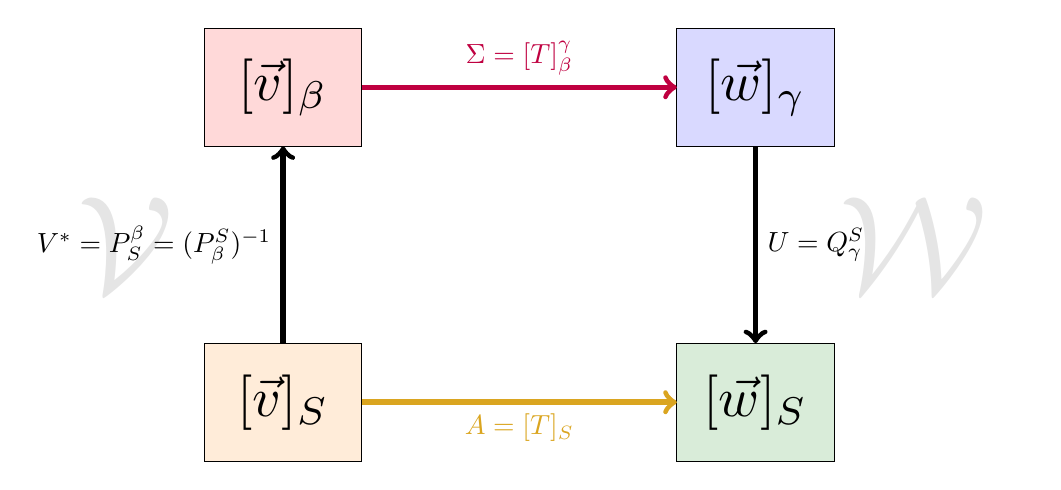
\begin{tikzpicture}
    \node[opacity=0.1,scale=5] at (-2,-2) {$\mathcal{V}$}; 
    \node[opacity=0.1,scale=5] at (8,-2) {$\mathcal{W}$};
    \draw [fill=red!15] (-1,-0.75) rectangle (1,0.75);
    \draw [fill=orange!15] (-1,-4.75) rectangle (1,-3.25);
    \draw [fill=blue!15] (5,-0.75) rectangle (7,0.75);
    \draw [fill=Green!15] (5,-4.75) rectangle (7,-3.25);
    \node[scale=2] at (0,0) {$[\vec{v}]_{\beta}$};
    \node[scale=2] at (6,0) {$[\vec{w}]_{\gamma}$};
    \node[scale=2] at (0,-4) {$[\vec{v}]_{S}$};
    \node[scale=2] at (6,-4) {$[\vec{w}]_{S}$}; 
    \draw[->, line width=2] (0,-3.25) -- (0,-0.75) node[midway, left]{$V^* = P_S^\beta = (P_{\beta}^S)^{-1}$};
    \draw[->, line width=2] (6,-0.75) -- (6,-3.25) node[midway, right]{$U = Q_{\gamma}^{S}$};
    \draw[purple, ->, line width=2] (1,0) -- (5,0) node[midway, above]{$\Sigma = [T]_\beta^\gamma$};
    \draw[Goldenrod, ->, line width=2] (1,-4) -- (5,-4) node[midway, below]{$A = [T]_S$};
    \end{tikzpicture}
    \caption{\textit{Same as Figure \ref{fig:transcoordsmatrix} but adapted to the context of SVD.}}
    \label{fig:transcoordSVD}
\end{figure}

\begin{exmp}
Find the SVD of the following $2 \times 3$ real matrix.
\begin{align*}
A &= 
\begin{bmatrix}
1 & 0 & 1\\
2 & 1 & 0
\end{bmatrix}
\end{align*}    
\end{exmp}
\begin{solution}
First, we compute its singular values, by considering the normal matrix:
\begin{align*}
A^TA &= 
\begin{bmatrix}
1 & 2\\
0 & 1 \\
1 & 0
\end{bmatrix} 
\begin{bmatrix}
1 & 0 & 1\\
2 & 1 & 0
\end{bmatrix} \\
&=
\begin{bmatrix}
5 & 2 & 1 \\
2 & 1 & 0 \\
1 & 0 & 1
\end{bmatrix}    
\end{align*}
which can be checked to have the eigenvalues of $\lambda = 6, 1, 0$, and hence $A$ has a decreasing sequence of singular values of $\sigma = \sqrt{6}, 1, 0$. The last singular value of zero is expected by Theorem \ref{thm:SVDtrans} and will be discarded. We note that the corresponding orthonormal eigenvectors for $A^TA$ are $\smash{(\frac{\sqrt{5}}{\sqrt{6}}, \frac{\sqrt{2}}{\sqrt{15}}, \frac{1}{\sqrt{30}})^T}$, $\smash{(0, -\frac{1}{\sqrt{5}}, \frac{2}{\sqrt{5}})^T}$, and $\smash{(-\frac{1}{\sqrt{6}}, \frac{2}{\sqrt{6}}, \frac{1}{\sqrt{6}})^T}$ and the readers can verify them. So we have
\begin{align*}
&V =
\left[\begin{array}{@{\,}wc{13pt}wc{13pt}wc{13pt}@{\,}}
\frac{\sqrt{5}}{\sqrt{6}} & 0 & -\frac{1}{\sqrt{6}}\\
\frac{\sqrt{2}}{\sqrt{15}} & -\frac{1}{\sqrt{5}} & \frac{2}{\sqrt{6}}\\
\frac{1}{\sqrt{30}} & \frac{2}{\sqrt{5}} & \frac{1}{\sqrt{6}}
\end{array}\right]
&\Sigma =
\begin{bmatrix}
\sqrt{6} & 0 & 0 \\
0 & 1 & 0
\end{bmatrix}
\end{align*}
The two column vectors for $U$ are found by
\begin{align*}
\hat{u}^{(1)} &= \frac{1}{\sigma_1} A\hat{v}^{(1)} \\
&= \frac{1}{\sqrt{6}}
\begin{bmatrix}
1 & 0 & 1\\
2 & 1 & 0
\end{bmatrix}
\begin{bmatrix}
\frac{\sqrt{5}}{\sqrt{6}} \\
\frac{\sqrt{2}}{\sqrt{15}} \\
\frac{1}{\sqrt{30}}
\end{bmatrix} \\
&=
\begin{bmatrix}
\frac{1}{\sqrt{5}} \\
\frac{2}{\sqrt{5}}
\end{bmatrix}
\end{align*}
and
\begin{align*}
\hat{u}^{(2)} &= \frac{1}{\sigma_2} A\hat{v}^{(2)} \\ 
&= \frac{1}{1}
\begin{bmatrix}
1 & 0 & 1\\
2 & 1 & 0
\end{bmatrix}
\begin{bmatrix}
0 \\
-\frac{1}{\sqrt{5}} \\
\frac{2}{\sqrt{5}}
\end{bmatrix} \\
&= 
\begin{bmatrix}
\frac{2}{\sqrt{5}} \\
-\frac{1}{\sqrt{5}}
\end{bmatrix}
\end{align*}
Therefore, we conclude that
\begin{align*}
U &=
\begin{bmatrix}
\frac{1}{\sqrt{5}} & \frac{2}{\sqrt{5}} \\
\frac{2}{\sqrt{5}} & -\frac{1}{\sqrt{5}}
\end{bmatrix} \\
A &= U\Sigma V^T \\
&= 
\begin{bmatrix}
\frac{1}{\sqrt{5}} & \frac{2}{\sqrt{5}} \\
\frac{2}{\sqrt{5}} & -\frac{1}{\sqrt{5}}
\end{bmatrix}
\begin{bmatrix}
\sqrt{6} & 0 & 0 \\
0 & 1 & 0
\end{bmatrix}
\left[\begin{array}{@{\,}wc{13pt}wc{13pt}wc{13pt}@{\,}}
\frac{\sqrt{5}}{\sqrt{6}} & \frac{\sqrt{2}}{\sqrt{15}} & \frac{1}{\sqrt{30}} \\
0 & -\frac{1}{\sqrt{5}} & \frac{2}{\sqrt{5}} \\
-\frac{1}{\sqrt{6}} & \frac{2}{\sqrt{6}} & \frac{1}{\sqrt{6}}
\end{array}\right]
=
\begin{bmatrix}
5 & 2 & 1 \\
2 & 1 & 0 \\
1 & 0 & 1
\end{bmatrix} 
\end{align*}
\end{solution}

\begin{exmp}
Carry out SVD for the $3 \times 2$ matrix below.
\begin{align*}
A =
\begin{bmatrix}
1 & 1 \\
0 & 1 \\
1 & 0
\end{bmatrix}
\end{align*}
\end{exmp}
\begin{solution}
We leave it to the readers to check that the two orthonormal eigenvectors of 
\begin{align*}
A^TA = 
\begin{bmatrix}
2 & 1 \\
1 & 2
\end{bmatrix}
\end{align*}
are 
\begin{align*}
& \hat{v}^{(1)} =
\begin{bmatrix}
\frac{1}{\sqrt{2}} \\
\frac{1}{\sqrt{2}}
\end{bmatrix}
& \hat{v}^{(2)} =
\begin{bmatrix}
-\frac{1}{\sqrt{2}} \\
\frac{1}{\sqrt{2}}
\end{bmatrix}
\end{align*}
for $\lambda_1 = 3$, $\lambda_2 = 1$, so $\sigma_1 = \sqrt{3}$, $\sigma_2 = 1$, and
\begin{align*}
\Sigma =
\begin{bmatrix}
\sqrt{3} & 0 \\
0 & 1 \\
0 & 0
\end{bmatrix}   
\end{align*}
$\hat{u}^{(1)}$, $\hat{u}^{(2)}$ are then given by
\begin{align*}
\hat{u}^{(1)} &= \frac{1}{\sigma_1} A\hat{v}^{(1)} = \frac{1}{\sqrt{3}}
\begin{bmatrix}
1 & 1 \\
0 & 1 \\
1 & 0
\end{bmatrix}
\begin{bmatrix}
\frac{1}{\sqrt{2}} \\
\frac{1}{\sqrt{2}}
\end{bmatrix}
=
\begin{bmatrix}
\frac{2}{\sqrt{6}} \\
\frac{1}{\sqrt{6}} \\
\frac{1}{\sqrt{6}} 
\end{bmatrix} \\
\hat{u}^{(2)} &= \frac{1}{\sigma_2} A\hat{v}^{(2)} = \frac{1}{1}
\begin{bmatrix}
1 & 1 \\
0 & 1 \\
1 & 0
\end{bmatrix}
\begin{bmatrix}
-\frac{1}{\sqrt{2}} \\
\frac{1}{\sqrt{2}}
\end{bmatrix}
=
\begin{bmatrix}
0 \\
\frac{1}{\sqrt{2}} \\
-\frac{1}{\sqrt{2}} 
\end{bmatrix}
\end{align*}
We need another unit vector $\hat{u}^{(3)}$ that is orthogonal to both $\hat{u}^{(1)}$ and $\hat{u}^{(2)}$. A quick way for this special case of three-dimensional vectors is to find the cross product $\hat{u}^{(1)} \times \hat{u}^{(2)}$, that is
\begin{align*}
\hat{u}^{(3)} &= \hat{u}^{(1)} \times \hat{u}^{(2)} =
\left|\begin{array}{@{\,}wc{13pt}wc{13pt}wc{13pt}@{\,}}
\hat{\imath} & \hat{\jmath} & \hat{k} \\
\frac{2}{\sqrt{6}} & \frac{1}{\sqrt{6}} & \frac{1}{\sqrt{6}}  \\
0 & \frac{1}{\sqrt{2}} & -\frac{1}{\sqrt{2}}
\end{array}\right|
= -\frac{1}{\sqrt{3}} \hat{\imath} + \frac{1}{\sqrt{3}} \hat{\jmath} + \frac{1}{\sqrt{3}} \hat{k}
=
\begin{bmatrix}
-\frac{1}{\sqrt{3}} \\
\frac{1}{\sqrt{3}} \\
\frac{1}{\sqrt{3}}
\end{bmatrix}
\end{align*} 
As a result,
\begin{align*}
U &=
\left[\begin{array}{@{\,}wc{13pt}wc{13pt}wc{13pt}@{\,}}
\frac{2}{\sqrt{6}} & 0 & -\frac{1}{\sqrt{3}} \\
\frac{1}{\sqrt{6}} & \frac{1}{\sqrt{2}} & \frac{1}{\sqrt{3}}\\
\frac{1}{\sqrt{6}} & -\frac{1}{\sqrt{2}} & \frac{1}{\sqrt{3}}
\end{array}\right] \\
A &= U\Sigma V^T \\
&= 
\left[\begin{array}{@{\,}wc{13pt}wc{13pt}wc{13pt}@{\,}}
\frac{2}{\sqrt{6}} & 0 & -\frac{1}{\sqrt{3}} \\
\frac{1}{\sqrt{6}} & \frac{1}{\sqrt{2}} & \frac{1}{\sqrt{3}}\\
\frac{1}{\sqrt{6}} & -\frac{1}{\sqrt{2}} & \frac{1}{\sqrt{3}}
\end{array}\right]
\begin{bmatrix}
\sqrt{3} & 0 \\
0 & 1 \\
0 & 0
\end{bmatrix} 
\begin{bmatrix}
\frac{1}{\sqrt{2}} & \frac{1}{\sqrt{2}}\\
-\frac{1}{\sqrt{2}} & \frac{1}{\sqrt{2}}
\end{bmatrix}
=
\begin{bmatrix}
1 & 1 \\
0 & 1 \\
1 & 0
\end{bmatrix}
\end{align*}
\end{solution}

\subsection{Geometric Perspective of SVD}

As discussed above, SVD involves two orthogonal/unitary coordinate transformations indicated by the matrices $U$ and $V$, one before and one after the mapping via the diagonal matrix $\Sigma$. In the case where $A$ happens to be a square matrix so that $m=n$ and if the vector spaces $\mathcal{V}$ and $\mathcal{W}$ have the same dimension and coincide, then from a geometric viewpoint, the action of $A$ can be separated into three steps: first a rotation/reflection, then a stretching/compression, finally followed by another rotation/reflection. We illustrate this using a small example. Consider
\begin{align*}
A = \begin{bmatrix}
1 & \frac{3}{2} \\
0 & 1
\end{bmatrix}
\end{align*}
which acts as a shear. It is not hard to obtain its SVD, which is noted below but the readers can try to derive it as a small exercise.
\begin{align*}
A = U \Sigma V^T
=
\begin{bmatrix}
\frac{2}{\sqrt{5}} & -\frac{1}{\sqrt{5}} \\
\frac{1}{\sqrt{5}} & \frac{2}{\sqrt{5}}
\end{bmatrix}
\begin{bmatrix}
2 & 0 \\
0 & \frac{1}{2}
\end{bmatrix}
\begin{bmatrix}
\frac{1}{\sqrt{5}} & \frac{2}{\sqrt{5}} \\
-\frac{2}{\sqrt{5}} & \frac{1}{\sqrt{5}}
\end{bmatrix}
\end{align*}
First, we have $V^T$ which constitutes a positive (counter-clockwise) rotation of the coordinate system by a degree of $\theta = \tan^{-1}(2) \approx \SI{63.4}{\degree}$ (see Section \ref{section:orthogeometricsub}). Then, the image is distorted by stretching/compressing along the intermediate $x$/$y$-axis respectively by a factor of $2$ through $\Sigma$. Finally, we carry out another coordinate frame rotation by a degree of $\theta = \tan^{-1}(1/2) \approx \SI{26.6}{\degree}$ in the negative (clockwise) direction. Notice that the passive rotations of the coordinate axes are equivalent to active rotations of vectors in the opposite sense. The flow of the entire procedure is shown in Figure \ref{fig:SVDgeometric} below.

\begin{figure}[ht!]
    \centering
    \begin{tikzpicture}
    \coordinate (0) at (0,0);
    \draw[thick] (0,0) circle (1.5);
    \draw[Green, ->] (0,0) -- (1.5,0) node[right](vecu){$\hat{e}^{(1)} = (1,0)^T$};
    \draw[red, ->] (0,0) -- (0.6708,1.3416) node[above right](vecv){$\hat{v}^{(1)}$};
    \draw[Green, ->] (0,0) -- (0,1.5) node[above left]{$\hat{e}^{(2)} = (0,1)^T$};
    \draw[red, ->] (0,0) -- (-1.3416,0.6708) node[above left]{$\hat{v}^{(2)}$};
    \pic[draw, ->, gray, "$\SI{63.4}{\degree}$", angle eccentricity=2.25] {angle = vecu--0--vecv};
    \draw[thick] (0,-4) circle (1.5);
    \draw[red, ->] (0,-4) -- (1.5,-4) node[right]{$x'$-axis};
    \draw[Green, ->] (0,-4) -- (0.6708,-1.3416-4);
    \draw[red, ->] (0,-4) -- (0,-2.5) node[above]{$y'$-axis};
    \draw[Green, ->] (0,-4) -- (1.3416,0.6708-4);
    \draw[thick] (6,-4) ellipse (3 and 0.75);
    \draw[blue, ->] (6,-4) -- (9,-4) node[midway, below]{Stretched ($\times 2$)};
    \draw[blue, ->] (6,-4) -- (6,-3.25) node[above]{Compressed ($\times \frac{1}{2}$)};
    \draw[Green, ->] (6,-4) -- (6+0.6708*2,-1.3416/2-4);
    \draw[Green, ->] (6,-4) -- (6+1.3416*2,0.6708/2-4);
    \draw[rotate around={26.6:(6,0)}, thick] (6,0) ellipse (3 and 0.75);
    \draw[Green, ->] (6,0) -- (7.5,0) node[below, xshift=16, yshift=-4]{$A\hat{e}^{(1)} = (1,0)^T$};
    \draw[Green, ->] (6,0) -- (8.25,1.5) node[above left, yshift=-2]{$A\hat{e}^{(2)} = (\frac{3}{2},1)^T$};
    \draw[blue, ->] (6,0) -- (6+1.3416*2,0.6708*2); 
    \draw[blue, ->] (6,0) -- (6-0.6708/2,1.3416/2);
    \draw[->] (-2,0) -- (-2,-4) node[midway, left]{$V^T$};
    \draw[->] (9,-3) -- (9,-1) node[midway, right]{$U$};
    \draw[->] (0,2.5) -- (6,2.5) node[midway, above]{$A$};
    \draw[->] (0,-6) -- (6,-6) node[midway, above]{$\Sigma$};
    \draw[gray, ->] (1,2-4) to [out=-22,in=108] (2,0.8-4) node[above right, yshift=2]{$\SI{63.4}{\degree}$};
    \draw[gray, ->] (5,-1.75) to [out=10, in=220, looseness=0.7] (7,-0.85) node[below, xshift=3, yshift=-5]{$\SI{26.6}{\degree}$};
    \end{tikzpicture}
    \caption{\textit{The geometric interpretation of the $2 \times 2$ SVD example. Red/Blue arrows represent the intermediate coordinate axes and green arrows mark the distortion of two given points indicated by the standard unit vectors initially.}}
    \label{fig:SVDgeometric}
\end{figure}


\subsection{Compact SVD}

During the derivation of Theorem \ref{thm:SVDtrans}, we have shown that if $n > m$ then there will be at least $n-m$ zero eigenvalues for $T^\dag T$ (or $A^*A$) in Footnote \ref{foot:zerosingular}. Of course, they are not included in the $\Sigma$ matrix as the main diagonal only has the length of $m$ so there will be $m$ singular values only. However, we can tighten the upper bound on the number of non-zero eigenvalues and therefore that of singular values. By the same Properties \ref{proper:AdagArank} used in Footnote \ref{foot:zerosingular}, we can know that if $A$ has a rank of $k \leq \min(m,n)$, then $A^*A$ will also have a rank of $k$ and thus $k$ non-zero singular values.\footnote{The rank of $k$ means that the nullity of $A^*A$ is $n-k$ by the Rank-nullity Theorem \ref{thm:ranknullity} and thus it has $n-k$ zero eigenvalues and thus $k$ non-zero eigenvalues (we implicitly have used Properties \ref{proper:symnodefic}, adapted for complex matrices, can you see how?).} Hence the original SVD of a rank $k$ matrix
\begin{align}
&\quad A = U\Sigma V^T \nonumber \\
&= \begin{bmatrix}
\hat{u}^{(1)} | \hat{u}^{(2)} | \cdots | \hat{u}^{(k)} | \cdots | \hat{u}^{(m)}
\end{bmatrix}
\begin{bmatrix}
\sigma_1 & 0 & \cdots & 0 & 0 & \cdots \\
0 & \sigma_2 & & \\
\vdots & & \ddots &\\
0 & & & \sigma_k & \\
0 & & & & 0 & \\
\vdots & & & & & \ddots
\end{bmatrix}
\left[\begin{array}{c} 
\hat{v}^{(1)*} \\
\hline
\hat{v}^{(2)*} \Tstrut \\
\hline
\vdots \\
\hline 
\hat{v}^{(k)*} \Tstrut \\
\hline
\vdots \\
\hline
\hat{v}^{(n)*} \Tstrut
\end{array}\right] 
\end{align}
can be reduced to the so-called \index{Truncated SVD}\index{Compact SVD}\keywordhl{Truncated/Compact SVD}, by only keeping entries associated with up to the first $k$ non-zero singular values, resulting in
\begin{align}
A = U_k\Sigma_k V_k^* = \begin{bmatrix}
\hat{u}^{(1)} | \hat{u}^{(2)} | \cdots | \hat{u}^{(k)}
\end{bmatrix}
\begin{bmatrix}
\sigma_1 & 0 & \cdots & 0 \\
0 & \sigma_2 & & \\
\vdots & & \ddots & \\
0 & & & \sigma_k
\end{bmatrix}
\left[\begin{array}{c} 
\hat{v}^{(1)*} \\
\hline
\hat{v}^{(2)*} \Tstrut \\
\hline
\vdots \\
\hline 
\hat{v}^{(k)*} \Tstrut 
\end{array}\right] 
\end{align}
where $U_k$, $V_k$ come from retaining only the first $k$ columns of $U$ and $V$, and $\Sigma_k$ is a diagonal $k \times k$ square matrix that preserves the $k$ non-zero singular values. From this point onwards, we mean the Compact SVD instead of the original one whenever we refer to SVD unless otherwise specified. If the singular values are distinct, the compact SVD of a matrix will be \textit{unique up to a (complex) sign difference}\footnote{which means that an $e^{i\theta}$ factor can be added to any singular vector.} for the singular vectors because the right singular vectors are designated to be the eigenvectors of $A^*A$ and we have required them to be arranged in the order of decreasing singular values. It can also be expanded in a fashion similar to Equation (\ref{eqn:projrank1sum}), which gives
\begin{align}
& \quad \begin{bmatrix}
\hat{u}^{(1)} | \hat{u}^{(2)} | \cdots | \hat{u}^{(k)}
\end{bmatrix}
\begin{bmatrix}
\sigma_1 & 0 & \cdots & 0 \\
0 & \sigma_2 & & \\
\vdots & & \ddots & \\
0 & & & \sigma_k
\end{bmatrix}
\left[\begin{array}{c} 
\hat{v}^{(1)*} \\
\hline
\hat{v}^{(2)*} \Tstrut \\
\hline
\vdots \\
\hline 
\hat{v}^{(k)*} \Tstrut 
\end{array}\right] \nonumber \\
&= \sigma_1\hat{u}^{(1)}\hat{v}^{(1)*} + \sigma_2\hat{u}^{(2)}\hat{v}^{(2)*} + \cdots + \sigma_k\hat{u}^{(k)}\hat{v}^{(k)*} 
\end{align}

\begin{exmp}
\label{exmp:compactSVD}
Find the (Compact) SVD of the following matrix.
\begin{align*}
A = 
\begin{bmatrix}
1&1&0&1\\ 
1&-1&1&0\\ 
2&0&1&1
\end{bmatrix}
\end{align*}
\end{exmp}
\begin{solution}
It is not hard to observe that the third row is the sum of the first two linearly independent rows so the rank of $A$ is $2$ (which can also be inferred from directly doing the Gaussian Elimination), so $A^TA$ also has a rank of $2$ and there will be two non-zero singular values for $A$. Now we compute the eigenvectors of $A^T A$ as usual, where the results are simply noted below:
\begin{align*}
A^TA = 
\begin{bmatrix}
6&0&3&3\\ 
0&2&-1&1\\ 
3&-1&2&1\\ 
3&1&1&2
\end{bmatrix}
\end{align*}
and
\begin{align*}
\vec{v}^{(1)} &= 
\left[\begin{array}{wc{10pt}}
\frac{2}{\sqrt{6}} \\
0 \\
\frac{1}{\sqrt{6}} \\
\frac{1}{\sqrt{6}}
\end{array}\right]
& \text{ for } \lambda_1 = 9 \\
\vec{v}^{(2)} &= 
\left[\begin{array}{wc{10pt}}
0 \\
\frac{2}{\sqrt{6}} \\
-\frac{1}{\sqrt{6}} \\
\frac{1}{\sqrt{6}}
\end{array}\right]
& \text{ for } \lambda_2 = 3 \\
\end{align*}
and $\vec{v}^{(3)} = \smash{(-\frac{1}{\sqrt{6}},\frac{1}{\sqrt{6}},\frac{2}{\sqrt{6}},0)^T}$, $\vec{v}^{(4)} = \smash{(-\frac{1}{\sqrt{6}},-\frac{1}{\sqrt{6}},0,\frac{2}{\sqrt{6}})^T}$ for $\lambda_3 = \lambda_4 = 0$. We now only need the first two of them for the SVD, so
\begin{align*}
V &= 
\begin{bmatrix}
\frac{2}{\sqrt{6}} & 0 \\
0 & \frac{2}{\sqrt{6}} \\
\frac{1}{\sqrt{6}} & -\frac{1}{\sqrt{6}}\\
\frac{1}{\sqrt{6}} & \frac{1}{\sqrt{6}}   
\end{bmatrix}
& \text{and} & &
\Sigma =
\begin{bmatrix}
3 & 0 \\
0 & \sqrt{3}
\end{bmatrix}
\end{align*}
as $\sigma_1 = \sqrt{\lambda_1} = \sqrt{9} =3$ and $\sigma_2 = \sqrt{\lambda_2} = \sqrt{3}$. Then we have
\begin{align*}
\vec{u}^{(1)} &= \frac{1}{\sigma_1} A\hat{v}^{(1)} \\
&= \frac{1}{3}\begin{bmatrix}
1&1&0&1\\ 
1&-1&1&0\\ 
2&0&1&1
\end{bmatrix}
\left[\begin{array}{wc{10pt}}
\frac{2}{\sqrt{6}} \\
0 \\
\frac{1}{\sqrt{6}} \\
\frac{1}{\sqrt{6}}
\end{array}\right] =
\left[\begin{array}{wc{10pt}}
\frac{1}{\sqrt{6}}\\ 
\frac{1}{\sqrt{6}}\\ 
\frac{2}{\sqrt{6}}
\end{array}\right]
\end{align*}
and
\begin{align*}
\vec{u}^{(2)} &= \frac{1}{\sigma_2} A\hat{v}^{(2)} \\
&= \frac{1}{\sqrt{3}}\begin{bmatrix}
1&1&0&1\\ 
1&-1&1&0\\ 
2&0&1&1
\end{bmatrix}
\left[\begin{array}{wc{10pt}}
0 \\
\frac{2}{\sqrt{6}} \\
-\frac{1}{\sqrt{6}} \\
\frac{1}{\sqrt{6}}
\end{array}\right] =
\left[\begin{array}{wc{10pt}}
\frac{1}{\sqrt{2}}\\ 
-\frac{1}{\sqrt{2}}\\ 
0
\end{array}\right]
\end{align*}
So
\begin{align*}
U = 
\begin{bmatrix}
\frac{1}{\sqrt{6}} & \frac{1}{\sqrt{2}}\\  
\frac{1}{\sqrt{6}} & -\frac{1}{\sqrt{2}}\\ 
\frac{2}{\sqrt{6}} & 0
\end{bmatrix}
\end{align*}
and it is not hard to check that
\begin{align*}
A &= U\Sigma V^* \\
\begin{bmatrix}
1&1&0&1\\ 
1&-1&1&0\\ 
2&0&1&1
\end{bmatrix} &=
\begin{bmatrix}
\frac{1}{\sqrt{6}} & \frac{1}{\sqrt{2}}\\  
\frac{1}{\sqrt{6}} & -\frac{1}{\sqrt{2}}\\ 
\frac{2}{\sqrt{6}} & 0
\end{bmatrix}
\begin{bmatrix}
3 & 0 \\
0 & \sqrt{3}
\end{bmatrix}
\begin{bmatrix}
\frac{2}{\sqrt{6}} & 0 & \frac{1}{\sqrt{6}} & \frac{1}{\sqrt{6}} \\
0 & \frac{2}{\sqrt{6}} & -\frac{1}{\sqrt{6}} & \frac{1}{\sqrt{6}} 
\end{bmatrix}
\end{align*}
\end{solution}

\subsection{Relation between SVD and PCA}

We will end this section by talking about how SVD can be used to carry out PCA, introduced in Section \ref{subsection:PCA}. Given a real data matrix $[X']$, PCA requires us to compute the eigenvalues and orthonormal eigenvectors of the covariance matrix $Q = \frac{1}{m-1}[X']^T[X']$ where $m$ is the number of data. If we know that the SVD of the data matrix is $[X'] = U\Sigma V^T$, then we have
\begin{align}
Q &= \frac{1}{m-1}[X']^T[X'] \nonumber \\
&= \frac{1}{m-1}(U\Sigma V^T)^TU\Sigma V^T \nonumber \\
&= \frac{1}{m-1}V \Sigma U^T U \Sigma V^T & \text{($\Sigma$ is diagonal)} \nonumber \\
&= \frac{1}{m-1}V \Sigma^2 V^T & \begin{aligned}
&\text{($U^TU = I$ as $U$ is orthogonal,} \\
&\text{Properties \ref{proper:orthoinvT})}
\end{aligned}\nonumber \\
&= V(\frac{\Sigma^2}{m-1}) V^T 
\end{align}
By comparing this to (\ref{eqn:orthodiagonalPAP}) in Definition \ref{defn:orthodiagonal}, we immediately identify that the orthogonal matrix $P = V$ contains the orthonormal principal directions in columns, which coincide with the right singular vectors of $[X']$. The variances of the PCs are related to the singular values by 
\begin{align}
\lambda_j = \frac{\sigma_j^2}{m-1}    
\end{align} as $D = \Sigma^2/(m-1)$. In addition, as suggested by (\ref{eqn:PCAcoordchange}) below Theorem \ref{thm:PCA}, the new PC coordinates are given \begin{align}
\vec{u}_i = [\textbf{e}]^T \vec{x}_i = V^T \vec{x}_i    
\end{align}
More generally, considering the entire data matrix $[X'] = [\vec{x}^{(1)}|\vec{x}^{(2)}|\cdots|\vec{x}^{(n)}]$ where each row represents a data point, we can compute the PCs for all data by
\begin{align}
V^TX^T &= V^T[\vec{x}^{(1)}|\vec{x}^{(2)}|\cdots|\vec{x}^{(n)}]^T = V^T
\begin{bmatrix}
x^{(1)}_1 & x^{(1)}_2 & \cdots & x^{(1)}_m \\
x^{(2)}_1 & x^{(2)}_2 & \cdots & x^{(2)}_m \\
\vdots & \vdots & & \vdots \\
x^{(n)}_1 & x^{(n)}_2 & \cdots & x^{(n)}_m
\end{bmatrix} \nonumber \\
&= V^T(U\Sigma V^T)^T \nonumber \\
&= V^TV \Sigma U^T = \Sigma U^T
\end{align}
and now each column of $\Sigma U^T$, or equivalently each row of $U\Sigma$, contains the PC coordinates of the corresponding data point. The readers are referred to \href{https://stats.stackexchange.com/questions/134282/relationship-between-svd-and-pca-how-to-use-svd-to-perform-pca}{this Statistics Stackexchange post} (134282) for a more in-depth explanation.

\section{Pseudoinverses}

\subsection{Definition of Pseudoinverses and Inference from SVD}

The Singular Value Theorem \ref{thm:SVDtrans} shows that a linear transformation can be described by Equation (\ref{eqn:SVDT}) between the orthonormal bases for $\mathcal{V}$ and $\mathcal{W}$. Particularly, for any non-zero singular value $\sigma_j > 0$, Equation (\ref{eqn:SVDT}) can be inverted as
\begin{align}
T^+(\vec{u}^{(j)}) = \frac{1}{\sigma_j} \vec{v}^{(j)} \label{eqn:pinv1}
\end{align}
where now $T^+$ reverts the mapping by $T$ from each of $\gamma = \{\vec{u}^{(1)}, \vec{u}^{(2)},\ldots,\vec{u}^{(k)}\}$ back to each of $\beta = \{\vec{v}^{(1)}, \vec{v}^{(2)},\ldots,\vec{v}^{(k)}\}$ where there are $k$ non-zero singular values. Notice that the subspaces generated by $\beta$ and $\gamma$ are the kernel's complement and the range, $\mathcal{N}(T)^\perp$ and $\mathcal{R}(T)$ respectively. Motivated by all of these, we may want to construct a \index{Pseudoinverse}\keywordhl{"pseudoinverse"} $T^+: \mathcal{W} \to \mathcal{V}$ out of $T$ even though the matrix representation of $T$ may not have a square shape to be invertible in the usual sense: we only need Equation (\ref{eqn:pinv1}) to hold from $\mathcal{R}(T)$ to $\mathcal{N}(T)^\perp$ and this will be good enough to capture the invertibility between just these two subspaces. Both $\mathcal{R}(T)$ and $\mathcal{N}(T)^\perp$ have the same dimension\footnote{Let $T$ has a rank of $k$ so that $\dim(\mathcal{R}(T)) = k$, then by the Rank-Nullity Theorem \ref{thm:ranknullitytrans}, $\dim(\mathcal{N}(T)) = n-k$ and $\dim(\mathcal{N}(T)^\perp) = n-(n-k) = k$.} and there will always be an invertible linear transformation $L$ between them by Properties \ref{proper:isomorphicsamerank}. We require that this $L$ coincides with $T$ as long as the input vectors are in the kernel's complement $\mathcal{N}(T)^\perp$ and hence in the backward direction $T^+$ coincides with $L^{-1}$ over the range $\mathcal{R}(T)$ as well. For other vectors in the complement of the range $\mathcal{R}(T)^\perp \subseteq \mathcal{W}$, we effectively ignore them by requiring that $T^+$ maps all of them into the zero vector. From these, we can properly define the pseudoinverse of a linear transformation as below.
\begin{defn}[Pseudoinverse of a Linear Transformation]
\label{defn:pseudoinversetrans}
For two inner product spaces $\mathcal{V}$ and $\mathcal{W}$ of finite dimensions $n$ and $m$ respectively, and given a linear transformation $T\colon \mathcal{V} \to \mathcal{W}$ between them, let $L\colon \mathcal{N}(T)^\perp \to \mathcal{R}(T)$ be the invertible linear transformation between the two subspaces $\mathcal{N}(T)^\perp$ and $\mathcal{R}(T)$ such that 
\begin{align}
L(\vec{v}) &= T(\vec{v}) & \text{ for every } \vec{v} \in \mathcal{N}(T)^\perp   
\end{align}
Then the \index{Moore-Penrose Pseudoinverse}\textit{(Moore-Penrose) pseudoinverse} $T^+: \mathcal{W} \to \mathcal{V}$ is defined by
\begin{align}
T^+(\vec{w}) = \begin{cases}
L^{-1}(\vec{w}) & \text{for $\vec{w} \in \mathcal{R}(T)$} \\
\textbf{0} & \text{for $\vec{w} \in \mathcal{R}(T)^\perp$} \\
\end{cases}
\end{align}
\end{defn}
Hence, the pseudoinverse always exists for any $T$ by construction, regardless of whether $T$ is invertible or not. Further, if $T$ is invertible, then we simply have $T^+ = T^{-1}$ as $\mathcal{N}(T)^\perp = \mathcal{V}$ and $\mathcal{R}(T) = \mathcal{W}$. Finally, the Moore-Penrose pseudoinverse, as a linear transformation, is also unique. Since the Singular Value Theorem can be translated to SVD for matrices, we may like to know if there will be a matrix version of the pseudoinverse as well. Remember that in SVD (Theorem \ref{thm:SVD}) the key is to transform the coordinate system from the standard basis to the $\beta$ basis through the matrix $V^*$, then apply the factors $\sigma_j$ through $\Sigma$, and finally transform the coordinate system again from the $\gamma$ basis back to the standard basis via the matrix $U$. Therefore, it is logical to derive the pseudoinverse matrix by reversing these three steps. We only need to take special care when we invert the middle step involving the sigma factors $\Sigma$: In the corresponding $\Sigma^+$ matrix, the first $k$ diagonal entries will be the reciprocals $1/\sigma_j$ for the $k$ non-zero singular values, and beyond that they will be all zeros so that any $\vec{w} \in \mathcal{R}(T)^\perp$ is indeed mapped to the zero vector. Subsequently, the pseudoinverse matrix will look like $A^+ = V\Sigma^+ U^*$
\begin{proper}[Pseudoinverse of a Matrix]
\label{proper:pinv}
Let $A$ be an $m \times n$ matrix with a (full) SVD of $A = U\Sigma V^*$ and $k \leq \min(m,n)$ non-zero singular values $\sigma_1 \geq \sigma_2 \geq \cdots \geq \sigma_k > 0$. Then, define a diagonal matrix $\Sigma^+$ where
\begin{align}
\Sigma^+_{ij} = \begin{cases}
\frac{1}{\sigma_j} & \text{if $i = j \leq k$} \\
0 & \text{otherwise}
\end{cases}
\end{align}
and the pseudoinverse of $A$ will then be 
\begin{align}
A^+ = V\Sigma^+ U^*    
\end{align}
\end{proper}
Note that we can also construct a "compact" pseudoinverse matrix just as the compact SVD by omitting the zero rows/columns of $\Sigma^+$, and the pseudoinverse matrix will also be unique up to a complex sign like the singular vectors themselves. In addition, the pseudoinverse of $\Sigma$ is simply $\Sigma^+$.

\begin{exmp}
\label{exmp:compactpinv}
Find the pseudoinverse of the matrix in Example \ref{exmp:compactSVD}.
\end{exmp}
\begin{solution}
Note that $U$ and $V$ are the same as in the original example, with
\begin{align*}
\Sigma^+ = 
\begin{bmatrix}
\frac{1}{3} & 0 \\
0 & \frac{1}{\sqrt{3}}
\end{bmatrix}
\end{align*}
Hence the pseudoinverse matrix is
\begin{align*}
A^+ &= V\Sigma^+ U^* \\
&=
\begin{bmatrix}
\frac{2}{\sqrt{6}} & 0 \\
0 & \frac{2}{\sqrt{6}} \\
\frac{1}{\sqrt{6}} & -\frac{1}{\sqrt{6}}\\
\frac{1}{\sqrt{6}} & \frac{1}{\sqrt{6}}   
\end{bmatrix}
\begin{bmatrix}
\frac{1}{3} & 0 \\
0 & \frac{1}{\sqrt{3}}
\end{bmatrix}
\begin{bmatrix}
\frac{1}{\sqrt{6}} & \frac{1}{\sqrt{6}} & \frac{2}{\sqrt{6}} \\  
\frac{1}{\sqrt{2}} & -\frac{1}{\sqrt{2}} & 0
\end{bmatrix} =
\begin{bmatrix}
\frac{1}{9}&\frac{1}{9}&\frac{2}{9}\\ 
\frac{1}{3}&-\frac{1}{3}&0\\ 
-\frac{1}{9}&\frac{2}{9}&\frac{1}{9}\\ 
\frac{2}{9}&-\frac{1}{9}&\frac{1}{9}
\end{bmatrix}
\end{align*}
\end{solution}
$\blacktriangleright$ Short Exercise: Check if (\ref{eqn:pinv1}) holds for the left singular vectors.\footnotemark\par
However, be reminded that in general, the product between a matrix and its pseudoinverse may not produce the identity matrix, i.e.\ $A^+ A \neq I$. Here, we have
\begin{align*}
A^+ A = 
\begin{bmatrix}
\frac{1}{9}&\frac{1}{9}&\frac{2}{9}\\ 
\frac{1}{3}&-\frac{1}{3}&0\\ 
-\frac{1}{9}&\frac{2}{9}&\frac{1}{9}\\ 
\frac{2}{9}&-\frac{1}{9}&\frac{1}{9}
\end{bmatrix}  
\begin{bmatrix}
1&1&0&1\\ 
1&-1&1&0\\ 
2&0&1&1
\end{bmatrix}
=
\begin{bmatrix}
\frac{2}{3}&0&\frac{1}{3}&\frac{1}{3}\\ 
0&\frac{2}{3}&-\frac{1}{3}&\frac{1}{3}\\ 
\frac{1}{3}&-\frac{1}{3}&\frac{1}{3}&0\\ 
\frac{1}{3}&\frac{1}{3}&0&\frac{1}{3}
\end{bmatrix}
\end{align*}
\footnotetext{We only check $\vec{u}^{(1)}$ here and leave $\vec{u}^{(2)}$ to the readers:
\begin{align*}
A^+\vec{u}^{(1)} = \begin{bmatrix}
\frac{1}{9}&\frac{1}{9}&\frac{2}{9}\\ 
\frac{1}{3}&-\frac{1}{3}&0\\ 
-\frac{1}{9}&\frac{2}{9}&\frac{1}{9}\\ 
\frac{2}{9}&-\frac{1}{9}&\frac{1}{9}
\end{bmatrix}
\begin{bmatrix}
\frac{1}{\sqrt{6}}\\ 
\frac{1}{\sqrt{6}}\\ 
\frac{2}{\sqrt{6}}    
\end{bmatrix}
=
\begin{bmatrix}
\frac{2}{3\sqrt{6}}\\ 
0\\ 
\frac{1}{3\sqrt{6}}\\ 
\frac{1}{3\sqrt{6}}
\end{bmatrix}
= \frac{1}{3}
\begin{bmatrix}
\frac{2}{\sqrt{6}}\\ 
0\\ 
\frac{1}{\sqrt{6}}\\ 
\frac{1}{\sqrt{6}}
\end{bmatrix}
= \frac{1}{\sigma_1}\vec{v}^{(1)}
\end{align*}}

\subsection{Minimal Solution}
\label{subsection:minsol}

One major usage of pseudoinverses is to compute the "best-fit" solution $\vec{x}_f$ for the system $A\vec{x} = \smash{\vec{h}}$ even if it has no solution (inconsistent) or infinitely many solutions, in the sense that the norm of $\vec{x}_f$ is minimized, and hence it is called the \index{Minimal Solution}\keywordhl{minimal solution}. As the name of pseudoinverses suggests, we can invert the system to acquire $\vec{x}_f = A^+\smash{\vec{h}}$ by treating $A^{+}$ just like the inverse of $A$. To show the minimal properties of $\vec{x}_f = A^+\smash{\vec{h}}$, we need to establish the following observations first.
\begin{proper}
\label{proper:minsollemma}
Let $\mathcal{V}$ and $\mathcal{W}$ be two finite-dimensional inner product spaces, and $T\colon \mathcal{V} \to \mathcal{W}$ be a linear transformation between them. Then
\begin{enumerate}[label=(\alph*)]
    \item $T^+ T$ is the orthogonal projection of $\mathcal{V}$ onto $\mathcal{N}(T)^\perp$;
    \item $T T^+$ is the orthogonal projection of $\mathcal{W}$ onto $\mathcal{R}(T)$.
\end{enumerate}
\end{proper}
\begin{proof}
Refer to Section \ref{subsection:orthoproj} for the definition of orthogonal projections. For (a), if $\vec{v} \in \mathcal{N}(T)^\perp$, then following Definition \ref{defn:pseudoinversetrans}, we have $T(\vec{v}) = L(\vec{v}) \in \mathcal{R}(T)$ and thus $T^+ T(\vec{v}) = L^{-1}(L(\vec{v})) = \vec{v}$. On the other hand, for $\vec{v} \in (\mathcal{N}(T)^\perp)^\perp = \mathcal{N}(T)$, we simply have $T^+ T(\vec{v}) = T^+(\textbf{0}) = \textbf{0}$. These two rules show that $T^+ T$ is the orthogonal projection of $\mathcal{V}$ onto $\mathcal{N}(T)^\perp$. The proof of (b) is similar and we leave it as an exercise to the readers.\footnote{Again by Definition \ref{defn:pseudoinversetrans}, for $\vec{v} \in \mathcal{R}(T)$, $T^+(\vec{v}) = L^{-1}(\vec{v})$ and $T T^+(\vec{v}) = L(L^{-1}(\vec{v})) = \vec{v}$. While for $\vec{v} \in \mathcal{R}(T)^\perp$, we have $T T^+(\vec{v}) = T(\textbf{0}) = \textbf{0}$.}
\end{proof} 
Now we are ready to show that $\vec{x}_f = A^+\smash{\vec{h}}$ is indeed the "best-fit" solution to $A\vec{x} = \vec{h}$ with the minimum norm.
\begin{proper}
\label{proper:minimalsoln}
For a linear system \smash{$A\vec{x} = \vec{h}$} where $A$ is an $m \times n$ matrix and \smash{$\vec{h}$} is a vector of length $m$, the proposed solution \smash{$\vec{x}_f = A^+\vec{h}$} will satisfy the following properties.
\begin{enumerate}[label=(\alph*)]
    \item If \smash{$A\vec{x} = \vec{h}$} is consistent, then $\vec{x}_f$ is the unique solution to the system such that it has the minimum norm possible, i.e.\ \smash{$A\vec{x}_f = \vec{h}$}, and \smash{$\norm{\smash{\vec{x}_f}} \leq \norm{\vec{x}}$} for any solution $\vec{x}$ to the system where the equality holds if and only if $\vec{x} = \vec{x}_f$;
    \item Otherwise, if \smash{$A\vec{x} = \vec{h}$} is inconsistent, then $\vec{x}_f$ is the unique best approximation to the solution of the system such that it still has the minimum norm possible, i.e.\ the error is minimized with \smash{$\norm{\smash{A\vec{x}_f - \vec{h}}} \leq \norm{\smash{A\vec{x} - \vec{h}}}$} for any $\vec{x}$ where the equality holds if and only if $A\vec{x} = A\vec{x}_f$. Furthermore, when there are multiple "best-fit" solutions $\vec{x}$ so that $A\vec{x} = A\vec{x}_f$, then \smash{$\norm{\smash{\vec{x}_f}} \leq \norm{\vec{x}}$} for where the equality holds if and only if $\vec{x} = \vec{x}_f$.
\end{enumerate}
\end{proper}
\begin{proof}
For (a), given $A\vec{x} = \smash{\vec{h}}$ is consistent, $\smash{\vec{h}}$ will be in the column space of $A$, $\mathcal{R}(A)$, by Properties \ref{proper:consistentcolspace}. So $A\vec{x}_f = AA^+\smash{\vec{h} = \vec{h}}$ by part (b) of Properties \ref{proper:minsollemma} where we set $T = A$, and thus $\vec{x}_f$ is indeed a solution to the linear system. For any solution $\vec{x}$ to $A\vec{x} = \smash{\vec{h}}$, we have
\begin{align*}
A^+A\vec{x} = A^+\vec{h} = \vec{x}_f
\end{align*}
and by part (a) of Properties \ref{proper:minsollemma}, it implies that $\vec{x}_f$ will be the orthogonal projection of $\vec{x}$ onto $\mathcal{N}(A)^\perp$. Using (\ref{eqn:shortestsubspacealta}) from Properties \ref{proper:shortestorthoproj} immediately shows that, the shortest norm $\norm{\vec{x}}$ where we fix $\vec{w} = \textbf{0}$ is achieved by $\vec{x}_f \in \smash{\mathcal{N}(A)^\perp}$ because
\begin{align*}
\norm{\vec{x}} = \norm{\vec{x} - \textbf{0}}^2 \geq \norm{T(\vec{x}) - \textbf{0}}^2 = \norm{\vec{x}_f - \textbf{0}}^2 = \norm{\vec{x}_f}^2     
\end{align*}
where $T = A^+A$ now. While for (b), if $A\vec{x} = \smash{\vec{h}}$ is inconsistent, then $A\vec{x}_f = AA^+\smash{\vec{h}}$ will be the orthogonal projection of $\smash{\vec{h}}$ onto $\mathcal{R}(A)$ by part (b) of Properties \ref{proper:minsollemma}. Therefore, using (\ref{eqn:shortestsubspacealtb}) this time in Properties \ref{proper:shortestorthoproj}, the minimum error $\norm{A\vec{x} - \smash{\vec{h}}}$ will be achieved by $\norm{T(\smash{\vec{h}}) - \smash{\vec{h}}} = \norm{AA^+\smash{\vec{h}} - \smash{\vec{h}}} = \norm{A\vec{x}_f - \smash{\vec{h}}}$ where we now take $T = AA^+$, $\vec{v} = \smash{\vec{h}}$ and $\mathcal{R}(A) = \mathcal{W}$. For any best-fit $\vec{x}$ that satisfies $A\vec{x} = A\vec{x}_f = \vec{y}$, multiplying both sides by $A^+$ to the left gives
\begin{align*}
A^+\vec{y} = A^+A\vec{x}_f = A^+A(A^+\vec{h}) = A^+\vec{h} = \vec{x}_f 
\end{align*}
The third equality holds because $A^+\smash{\vec{h}} \in \mathcal{N}(T)^\perp$ and $A^+A$ is the orthogonal projection onto $\mathcal{N}(T)^\perp$ by part (a) of Properties \ref{proper:minsollemma}. Therefore, applying part (a) of the current properties on the other linear system $A\vec{x} = \vec{y}$ and the proposed solution $\vec{x}_f = A^+\vec{y}$ immediately shows that the shortest norm $\norm{\vec{x}}$ with $\vec{x}$ still being the best approximation to the original equation $A\vec{x} = \smash{\vec{h}}$ such that $A\vec{x} = \vec{y}$, is achieved by $\norm{\vec{x}\smash{_f}} \leq \norm{\vec{x}}$.
\end{proof}

\begin{exmp}
\label{exmp:minsol2h}
Find the minimal solution of the system $A\vec{x} = \vec{h}$, where 
\begin{align*}
A = 
\begin{bmatrix}
1&1&0&1\\ 
1&-1&1&0\\ 
2&0&1&1
\end{bmatrix}
\end{align*}    
is the matrix from Example \ref{exmp:compactSVD}, and $\vec{h} = $ (a) $(2,0,2)^T$ and (b) $(1,1,1)^T$.
\end{exmp}
\begin{solution}
By Properties \ref{proper:minimalsoln}, we simply compute $A^+\vec{h}$ for both cases, where
\begin{align*}
A^+ =
\begin{bmatrix}
\frac{1}{9}&\frac{1}{9}&\frac{2}{9}\\ 
\frac{1}{3}&-\frac{1}{3}&0\\ 
-\frac{1}{9}&\frac{2}{9}&\frac{1}{9}\\ 
\frac{2}{9}&-\frac{1}{9}&\frac{1}{9}
\end{bmatrix}
\end{align*}
by Example \ref{exmp:compactpinv}. In (a), it can be checked that the system is consistent for the given $\vec{h}$, and
\begin{align*}
A^+\vec{h} = 
\begin{bmatrix}
\frac{1}{9}&\frac{1}{9}&\frac{2}{9}\\ 
\frac{1}{3}&-\frac{1}{3}&0\\ 
-\frac{1}{9}&\frac{2}{9}&\frac{1}{9}\\ 
\frac{2}{9}&-\frac{1}{9}&\frac{1}{9}
\end{bmatrix}
\begin{bmatrix}
2 \\
0 \\
2
\end{bmatrix}
=
\begin{bmatrix}
\frac{2}{3}\\ 
\frac{2}{3}\\
0\\ 
\frac{2}{3}
\end{bmatrix}
\end{align*}
It can be verified that this solves the linear system exactly. Meanwhile for (b), we have
\begin{align*}
A^+\vec{h} = 
\begin{bmatrix}
\frac{1}{9}&\frac{1}{9}&\frac{2}{9}\\ 
\frac{1}{3}&-\frac{1}{3}&0\\ 
-\frac{1}{9}&\frac{2}{9}&\frac{1}{9}\\ 
\frac{2}{9}&-\frac{1}{9}&\frac{1}{9}
\end{bmatrix}
\begin{bmatrix}
1 \\
1 \\
1
\end{bmatrix}  
=
\begin{bmatrix}
\frac{4}{9}\\ 
0\\ 
\frac{2}{9}\\ 
\frac{2}{9}
\end{bmatrix}
\end{align*}
and
\begin{align*}
A(A^+\vec{h}) = 
\begin{bmatrix}
1&1&0&1\\ 
1&-1&1&0\\ 
2&0&1&1
\end{bmatrix}
\begin{bmatrix}
\frac{4}{9}\\ 
0\\ 
\frac{2}{9}\\ 
\frac{2}{9}
\end{bmatrix}
=
\begin{bmatrix}
\frac{2}{3} \\
\frac{2}{3} \\
\frac{4}{3}
\end{bmatrix}
\neq 
\begin{bmatrix}
1 \\
1 \\
1
\end{bmatrix} 
= \vec{h}
\end{align*}
The minimum error is $\norm{AA^+\vec{h} - \vec{h}} = \sqrt{\left(1-\frac{2}{3}\right)^2 + \left(1-\frac{2}{3}\right)^2 + \left(1-\frac{4}{3}\right)^2} = \frac{1}{\sqrt{3}}$.
\end{solution}
We note that the pseudoinverse solution coincides with the least-square solution in Theorem \ref{thm:bestfit} when the full SVD is employed:
\begin{align*}
\vec{x}_f &= (A^* A)^{-1}A^* \vec{h} \\
&= (V \Sigma^* U^* U\Sigma V^*)^{-1} (V \Sigma U^*) \vec{h} \\
&= (V \Sigma^* \Sigma V^*)^{-1} (V \Sigma U^*) \vec{h} & \text{(Definition \ref{defn:unitary}, $U$ is unitary)} \\
&= (V^*)^{-1} \Sigma^+ (\Sigma^+)^* V^{-1} V \Sigma U^* \vec{h} \\
&= V \Sigma^+ (\Sigma^+)^* \Sigma U^* \vec{h} & \text{(Definition \ref{defn:unitary}, $V$ is unitary)} \\
&= V {\Sigma^+} U^* \vec{h} = A^+\vec{h} & 
\begin{aligned}
\text{($(\Sigma^+)^* \Sigma = I$ if $m \geq n$} \\ \text{and $\Sigma$ is full-rank)} 
\end{aligned}
\end{align*}
as long as $A$ and thus $\Sigma$ are full-rank. Finally, by Properties \ref{proper:minsollemma}, we can arrive at the four equivalent defining properties of Moore-Penrose pseudoinverses as below.
\begin{proper}
\label{proper:pinvequiv}
An alternative set of definitions for the Moore-Penrose pseudoinverse $A^+$ of a matrix $A$ is
\begin{enumerate}
    \item $AA^+A = A$ ($A$ is a \index{Weak Inverse}\textit{weak inverse});
    \item $A^+AA^+ = A^+$ ($A^+$ is also a weak inverse);
    \item $(AA^+)^\dag = AA^+$ ($AA^+$ is Hermitian);
    \item $(A^+A)^\dag = A^+A$ ($A^+A$ is also Hermitian).
\end{enumerate}
\end{proper}
The first condition can be inferred as follows. $A\vec{v} \in \mathcal{R}(A)$ is in the column space of $A$ for any $\vec{v}$, and thus $AA^+A\vec{v} = AA^+(A\vec{v}) = A\vec{v}$ as $AA^+$ is the orthogonal projection onto $\mathcal{R}(A)$ by (a) of Properties \ref{proper:minsollemma} and we must have $AA^+A = A$. The second condition is derived similarly. Finally, the last two conditions are the direct consequence of applying the part $T = T^\dag$ of Properties \ref{proper:orthoprojadjoint} to Properties \ref{proper:minsollemma} where $T = A^+A$ and $T= AA^+$ are both orthogonal projections.

\section{Generalization of SVD to Alternative Inner Products}
\label{section:SVDgeneral}

In the Singular Value Theorem \ref{thm:SVDtrans}, the adjoint $T^\dag$ of the linear transformation $T$ is involved, but for simplicity, during the derivation of the matrix SVD, we have only discussed the case where the conjugate transpose $A^*$ is used in place of the adjoint $A^\dag$. However, as already shown in Section \ref{section:adjointherm}, we can define different matrix adjoints with respect to different inner products, and hence different notions of orthogonality and distance. Therefore, one may ask if we can come up with a variant of matrix SVD and pseudoinverses that incorporates the symmetric/Hermitian bilinear form associated with any inner product, and for example, at the same time still produces orthonormal bases of left/right singular vectors. The answer is possible, with appropriate changes to the previous formulae about SVD while the essence of its properties remains intact. We now state the formulation below.

\begin{defn}[SVD for an Alternative Adjoint]
\label{defn:SVDadjoint}
For any $m \times n$ matrix $A$, its adjoint with respect to the two inner products defined by the symmetric/Hermitian bilinear forms $B$ and $C$ for $\mathbb{C}^m$ and $\mathbb{C}^n$, is
\begin{align}
A^\dag = C^{-1} A^* B \label{eqn:altadjoint}
\end{align}
(replace $A^*$ by $A^T$ for $\mathbb{R}^m$ and $\mathbb{R}^n$) Meanwhile, the new matrix SVD with respect to this adjoint is
\begin{align}
A = U\Sigma V^*C \label{eqn:SVDadjoint}
\end{align}
where $U$ and $V$ are $m \times m$ and $n \times n$ matrices, and $\Sigma$ is an $m \times n$ diagonal matrix. The matrix $V$ is constructed by
\begin{align}
V = 
\begin{bmatrix}
\hat{v}^{(1)} | \hat{v}^{(2)} | \cdots | \hat{v}^{(n)}
\end{bmatrix}
\end{align}
where the column vectors $\hat{v}^{(1)}, \hat{v}^{(2)}, \ldots, \hat{v}^{(n)}$ are the orthonormal (now with respect to the inner product described by $C$) eigenvectors of the Hermitian matrix product $A^\dag A$ (Properties \ref{proper:orthogonalherm}, also called the \keywordhl{right singular vectors} in this case), and ordered by decreasing, real (Properties 
\ref{proper:hermrealeiginner}) eigenvalues $\lambda_1 \geq \lambda_2 \geq \cdots \geq \lambda_n \geq 0$ as well. $\Sigma$ then consists of the first $k = \min(m,n)$ \keywordhl{singular values} $\sigma_j = \smash{\sqrt{\lambda_j}}$ which are the square roots of the eigenvalues of $A^\dag A$ (also in decreasing order) for these right singular vectors $\hat{v}^{(j)}$ in the (unitary, with respect to $C$) matrix $V$ along the main diagonal, and has a value of zero elsewhere. Finally, $U$ is made up of the orthonormal (with respect to the inner product described by $B$) column vectors that satisfy
\begin{align}
\hat{u}^{(j)} = \frac{1}{\sigma_j} A\hat{v}^{(j)} \label{eqn:leftsingadjoint}
\end{align}
for any $j$ that is associated with a non-zero singular value $\sigma_j \neq 0$. These vectors $\hat{u}^{(j)}$ are also called the \keywordhl{left singular vectors} in this case. Again, when there are not enough column vectors to construct $U$ by this relation, use Gram-Schmidt Orthogonalization (Definition \ref{defn:GSorthinner} adapted for the new inner product) to create orthonormal vectors that extend the basis of $\hat{u}^{(j)}$ up to $j = m$.
\end{defn}
\begin{defn}[Pseudoinverse of a Matrix for an Alternative Adjoint]
Let $A$ be an $m \times n$ matrix with the (full) SVD of $A = U\Sigma V^*C$ with respect to some adjoint $A^\dag$ as given in (\ref{eqn:SVDadjoint}) of Theorem \ref{defn:SVDadjoint} that has $k \leq \min(m,n)$ non-zero singular values $\sigma_1 \geq \sigma_2 \geq \cdots \geq \sigma_k > 0$. Then define a diagonal matrix $\Sigma^+$ where
\begin{align}
\Sigma^+_{ij} = \begin{cases}
\frac{1}{\sigma_j} & \text{if $i = j \leq k$} \\
0 & \text{otherwise}
\end{cases}
\end{align}
and the pseudoinverse of $A$ with respect to this adjoint will then be
\begin{align}
A^+ = V \Sigma^+ U^* B \label{eqn:pinvadjoint}
\end{align}
\end{defn}
It means that SVD and pseudoinverses with respect to alternative inner products require two major modifications. First, the singular vectors are derived from $A^\dag A$ instead of $A^* A$ and will be orthonormal with respect to these inner products instead of the usual Euclidean inner products. Second, the SVD and pseudoinverse will need an extra scaling by the bilinear forms $C$ and $B$ first. With these appropriate modifications, all the properties proposed in Section \ref{subsection:minsol} will continue to hold. Now let's see how we find the minimal solution of an inconsistent system when the norms and errors are defined with respect to other inner products different from the standard inner products.
\begin{exmp}
Find the minimal solution of the inconsistent system \smash{$A\vec{x} = \vec{h}$}, where 
\begin{align*}
A &= 
\begin{bmatrix}
1 & -1 & 2 \\
2 & -2 & 4
\end{bmatrix} 
& & \vec{h} =
\begin{bmatrix}
1 \\
3
\end{bmatrix}
\end{align*} 
where the error between $\vec{h}$ and $A\vec{x}$ is computed with respect to the inner product defined by
\begin{align*}
B &= 
\begin{bmatrix}
1 & 1 \\
1 & 2
\end{bmatrix} \\
\norm{\smash{A\vec{x} - \vec{h}}}^2 &= (A\textbf{x} - \textbf{h})^T B(A\textbf{x} - \textbf{h})
\end{align*}
and the norm $\norm{\vec{x}}$ is computed with respect to the inner product defined by
\begin{align*}
C &= 
\begin{bmatrix}
2 & 0 & 0 \\
0 & 2 & 1 \\
0 & 1 & 2
\end{bmatrix} \\
\norm{\vec{x}}^2 &= \textbf{x}^TC\textbf{x}
\end{align*}
\end{exmp}
\begin{solution}
By (\ref{eqn:altadjoint}), the new adjoint is
\begin{align*}
A^\dag &= C^{-1} A^* B \\
&= \begin{bmatrix}
2 & 0 & 0 \\
0 & 2 & 1 \\
0 & 1 & 2
\end{bmatrix}^{-1}
\begin{bmatrix}
1 & 2 \\
-1 & -2 \\
2 & 4
\end{bmatrix} 
\begin{bmatrix}
1 & 1 \\
1 & 2
\end{bmatrix} \\
&=
\begin{bmatrix}
\frac{3}{2} & \frac{5}{2}\\ 
-4 & -\frac{20}{3}\\ 
5 & \frac{25}{3}
\end{bmatrix}
\end{align*}
Then $A^\dag A$ is computed as
\begin{align*}
A^\dag A &= \begin{bmatrix}
\frac{3}{2} & \frac{5}{2}\\ 
-4 & -\frac{20}{3}\\ 
5 & \frac{25}{3}
\end{bmatrix}
\begin{bmatrix}
1 & -1 & 2 \\
2 & -2 & 4
\end{bmatrix} \\
&= \begin{bmatrix}
\frac{13}{2} & -\frac{13}{2} & 13\\ 
-\frac{52}{3} & \frac{52}{3} & -\frac{104}{3}\\ 
\frac{65}{3} & -\frac{65}{3} & \frac{130}{3}
\end{bmatrix}
\end{align*}
The only non-zero eigenvalue and eigenvector of $A^\dag A$ can be seen to be
\begin{align*} \vec{v}^{(1)} &=
\begin{bmatrix}
3\\ 
-8\\ 
10
\end{bmatrix} & & \text {for $\lambda_1 = \frac{403}{6}$}
\end{align*}
and hence the corresponding singular value and the normalized right singular vector (with respect to $C$) will be
\begin{align*} \hat{v}^{(1)} &= 
\begin{bmatrix}
\frac{3}{\sqrt{186}}\\ 
-\frac{8}{\sqrt{186}}\\ 
\frac{10}{\sqrt{186}}
\end{bmatrix} & & \text {for $\sigma_1 = \sqrt{\frac{403}{6}}$}
\end{align*}
The corresponding left singular vector is then derived according to (\ref{eqn:leftsingadjoint}) as
\begin{align*}
\hat{u}^{(1)} &= \frac{1}{\sigma_1} A\hat{v}^{(1)} \\    
&= \frac{1}{\sqrt{\frac{403}{6}}} \begin{bmatrix}
1 & -1 & 2 \\
2 & -2 & 4
\end{bmatrix} 
\begin{bmatrix}
\frac{3}{\sqrt{186}}\\ 
-\frac{8}{\sqrt{186}}\\ 
\frac{10}{\sqrt{186}}
\end{bmatrix} = \begin{bmatrix}
\frac{1}{\sqrt{13}} \\
\frac{2}{\sqrt{13}}
\end{bmatrix}
\end{align*}
Therefore, following (\ref{eqn:pinvadjoint}), the pseudoinverse $A^+$ with respect to the adjoint is constructed by (using only the compact part of its SVD) 
\begin{align*}
A^+ &= V \Sigma^+ U^* B \\
&= \hat{v}^{(1)} \left(\frac{1}{\sigma_1}\right) \hat{u}^{(1)*} B \\
&= \begin{bmatrix}
\frac{3}{\sqrt{186}}\\ 
-\frac{8}{\sqrt{186}}\\ 
\frac{10}{\sqrt{186}}
\end{bmatrix}
\left(\frac{1}{\sqrt{\frac{403}{6}}}\right)
\begin{bmatrix}
\frac{1}{\sqrt{13}} & \frac{2}{\sqrt{13}}
\end{bmatrix}
\begin{bmatrix}
1 & 1 \\
1 & 2
\end{bmatrix} =
\begin{bmatrix}
\frac{9}{403} & \frac{15}{403}\\ 
-\frac{24}{403} & -\frac{40}{403}\\ 
\frac{30}{403} & \frac{50}{403}
\end{bmatrix}
\end{align*}
and then the minimal solution as in Properties \ref{proper:minimalsoln} will be
\begin{align*}
\vec{x}_f &= A^+\vec{h} \\
&= \begin{bmatrix}
\frac{9}{403} & \frac{15}{403}\\ 
-\frac{24}{403} & -\frac{40}{403}\\ 
\frac{30}{403} & \frac{50}{403}
\end{bmatrix}
\begin{bmatrix}
1 \\
3
\end{bmatrix} =
\begin{bmatrix}
\frac{54}{403}\\ 
-\frac{144}{403}\\ 
\frac{180}{403}
\end{bmatrix}
\end{align*}
\end{solution}
$\blacktriangleright$ Short Exercise: Check if (1) (as well as (2)) in Properties \ref{proper:pinvequiv} holds in this example.\footnotemark

\section{Earth Science Applications}

\begin{exmp}
Find the minimal solution to the ion concentrations in the seawater sample in Example \ref{exmp:seaion}.
\end{exmp}
\begin{solution}
The linear system can be written as \smash{$A\vec{x} = \vec{h}$} where
\begin{align*}
A &= 
\begin{bmatrix}
1 & 2 & -1 & -2 \\
23.0 & 24.3 & 35.5 & 96.1    
\end{bmatrix}
& & \vec{h} =
\begin{bmatrix}
0 \\
34.0
\end{bmatrix}
\end{align*}
We first seek the SVD of the matrix $A$ as suggested by Theorem \ref{thm:SVD}. We have\footnotetext{We will only show (1) and leave (2) to the readers. Both of them are routine calculations.
\begin{align*}
AA^+A &= \begin{bmatrix}
1 & -1 & 2 \\
2 & -2 & 4
\end{bmatrix} 
\begin{bmatrix}
\frac{9}{403} & \frac{15}{403}\\ 
-\frac{24}{403} & -\frac{40}{403}\\ 
\frac{30}{403} & \frac{50}{403}
\end{bmatrix}
\begin{bmatrix}
1 & -1 & 2 \\
2 & -2 & 4
\end{bmatrix} \\
&=
\begin{bmatrix}
\frac{3}{13}&\frac{5}{13}\\ 
\frac{6}{13}&\frac{10}{13}
\end{bmatrix}
\begin{bmatrix}
1 & -1 & 2 \\
2 & -2 & 4
\end{bmatrix}
= 
\begin{bmatrix}
1 & -1 & 2 \\
2 & -2 & 4
\end{bmatrix}
= A
\end{align*}
}
\begin{align*}
A^TA &=
\begin{bmatrix}
1 & 23.0 \\
2 & 24.3 \\
-1 & 35.5 \\
-2 & 96.1    
\end{bmatrix}
\begin{bmatrix}
1 & 2 & -1 & -2 \\
23.0 & 24.3 & 35.5 & 96.1    
\end{bmatrix} \\
&=
\begin{bmatrix}
530&560.9&815.5&2208.3\\ 
560.9&594.49&860.65&2331.23\\ 
815.5&860.65&1261.25&3413.55\\ 
2208.3&2331.23&3413.55&9239.21
\end{bmatrix}
\end{align*}
It would be wise to delegate the calculation of the eigenvalues of $A^TA$ and thus the singular values of $A$ to a computer, and we simply note the results for the two non-zero singular values below.
\begin{align*}
\hat{v}^{(1)} &= 
\begin{bmatrix}
0.21325 \\
0.22518 \\  
0.32946 \\
0.89178
\end{bmatrix}
& \sigma_1 \approx 107.78 \\
\hat{v}^{(2)} &= 
\begin{bmatrix}
-0.46577 \\
-0.82773 \\
0.18590 \\
0.25171
\end{bmatrix}
& \sigma_2 \approx 2.81 
\end{align*}
and
\begin{align*}
\hat{u}^{(1)} &= \frac{1}{\sigma_1} A\hat{v}^{(1)} \\
&= \frac{1}{107.78} \begin{bmatrix}
1 & 2 & -1 & -2 \\
23.0 & 24.3 & 35.5 & 96.1    
\end{bmatrix}
\begin{bmatrix}
0.21325 \\
0.22518 \\  
0.32946 \\
0.89178
\end{bmatrix} = 
\begin{bmatrix}
-0.01345 \\
0.99991
\end{bmatrix} \\
\hat{u}^{(2)} &= \frac{1}{\sigma_2} A\hat{v}^{(2)} \\
&= \frac{1}{2.81} \begin{bmatrix}
1 & 2 & -1 & -2 \\
23.0 & 24.3 & 35.5 & 96.1    
\end{bmatrix}
\begin{bmatrix}
-0.46577 \\
-0.82773 \\
0.18590 \\
0.25171
\end{bmatrix} = 
\begin{bmatrix}
-0.99991 \\
-0.01345
\end{bmatrix}
\end{align*}
Hence according to Formula (\ref{eqn:pinvadjoint}) in Properties \ref{proper:pinv}, the pseudoinverse of $A$ is
\begin{align*}
A^+ &= V\Sigma^+ U^* \\
&= 
\begin{bmatrix}
0.21325 & -0.46577 \\
0.22518 & -0.82773 \\  
0.32946 & 0.18590 \\
0.89178 & 0.25171
\end{bmatrix}
\begin{bmatrix}
\frac{1}{107.78} & 0 \\
0 & \frac{1}{2.81}
\end{bmatrix}
\begin{bmatrix}
-0.01345 & 0.99991 \\
-0.99991 & -0.01345
\end{bmatrix} \\
&=
\begin{bmatrix}
0.1657 & 0.0042 \\
0.2944 & 0.0060 \\
-0.0662 & 0.0022 \\
-0.0897 & 0.0071 
\end{bmatrix}
\end{align*}
and thus the minimal solution will be
\begin{align*}
\vec{x}_f &= A^+\vec{h} \\
&= 
\begin{bmatrix}
0.1657 & 0.0042 \\
0.2944 & 0.0060 \\
-0.0662 & 0.0022 \\
-0.0897 & 0.0071 
\end{bmatrix}
\begin{bmatrix}
0 \\
34.0
\end{bmatrix}
=
\begin{bmatrix}
0.1430 \\
0.2057 \\
0.0737 \\
0.2403
\end{bmatrix}
\end{align*}
We can convert the molar concentration of each ion species to mass concentration via multiplying them by their respective molar mass. For example,
\begin{align*}
[\text{Na}^+] &= (\SI{23.0}{\g \per \mol})(\SI{0.1430}{\mol \per \kg}) = \SI{3.29}{\g \per \kg}
\end{align*}
and similarly $[\text{Mg}^{2+}] = (24.3)(0.2057) = \SI{5.00}{\g \per \kg}$, $[\text{Cl}^{-}] = (35.5)(0.0737) \allowbreak = \SI{2.62}{\g \per \kg}$, $[\text{SO}_4^{2-}] = (96.1)(0.2403) = \SI{23.09}{\g \per \kg}$. However, while this minimal solution is a valid solution by part (a) of Properties \ref{proper:minimalsoln}, it is far from the actual observed composition (see \href{https://www.britannica.com/science/seawater}{https://www.britannica.com/science/\\seawater}). This is because the minimal solution also tries to minimize the squared norm $\norm{\vec{x}}^2$, which tends to average out the components. Therefore, we have to be very careful if we attempt to obtain a single solution for a linear system that admits infinitely many solutions using the pseudoinverse.
\end{solution}

\section{Python Programming}
First, we will demonstrate how to carry out Cholesky Factorization and L(D)U Decomposition. We will take the matrices in Examples \ref{exmp:Cholesky} and \ref{exmp:PLU} for those.
\begin{lstlisting}
import numpy as np
from scipy import linalg

A1 = np.array([[4, 2, 0],
               [2, 2, 2],
               [0, 2, 5]])
print(linalg.cholesky(A1))
\end{lstlisting}
gives
\begin{lstlisting}
[[2. 1. 0.]
 [0. 1. 2.]
 [0. 0. 1.]]    
\end{lstlisting}
as expected, and
\begin{lstlisting}
A2 = np.array([[1, 1, 2],
               [2, 2, 3],
               [1, 3, 0]])
P, L, U_raw = linalg.lu(A2)
D = np.diag(np.diag(U_raw)) # Factor out the diagonal elements in U_raw
U = U_raw/np.diag(U_raw)[:,None]
print(P, L, D, U)
print(np.allclose(P@L@D@U, A2)) # Check if the factors can be combined to reconstruct the matrix
\end{lstlisting}
which produces
\begin{lstlisting}
[[0.  0.  1. ]
 [1.  0.  0. ]
 [0.  1.  0. ]] 
[[1.  0.  0.  ]
 [0.5 1.  0.  ]
 [0.5 0.  1.  ]] 
[[2.  0.  0.  ]
 [0.  2.  0.  ]
 [0.  0.  0.5 ]] 
[[1.  1.  1.5 ]
 [0.  1.  -0.75]
 [0.  0.  1.  ]]
True
\end{lstlisting}
as another valid outcome of (P)LDU Decomposition different from the one derived in Example \ref{exmp:PLU}. Now we will move to the central topic in this chapter, the Singular Value Decomposition (SVD). We are going to use Example \ref{exmp:compactSVD} to illustrate how to perform that. The results of
\begin{lstlisting}
A3 = np.array([[1, 1, 0, 1],
               [1,-1, 1, 0],
               [2, 0, 1, 1]])
U, Sigma, V_H = linalg.svd(A3) # can set the optional parameter full_matrices = False to obtain the compact SVD and increase speed
print(U, Sigma, V_H)
\end{lstlisting}
are
\begin{lstlisting}
[[-4.08248290e-01 -7.07106781e-01 -5.77350269e-01]
 [-4.08248290e-01  7.07106781e-01 -5.77350269e-01]
 [-8.16496581e-01  2.22044605e-16  5.77350269e-01]] 
 [3.00000000e+00 1.73205081e+00 9.06493304e-17] 
[[-8.1649658e-01 -1.1102230e-16 -4.0824829e-01 -4.0824829e-01]
 [ 2.2204460e-16 -8.1649658e-01  4.0824829e-01 -4.0824829e-01]
 [-4.8232914e-02 -5.7533200e-01 -5.2709909e-01  6.2356492e-01]]    
\end{lstlisting}
which essentially matches the full SVD of the matrix where the extremely small values are actually zeros but affected by numerical round-off errors, and there are some sign differences. The pseudoinverse can be simply computed by
\begin{lstlisting}
print(linalg.pinv(A3))
\end{lstlisting}
that returns
\begin{lstlisting}
[[ 1.11111111e-01  1.11111111e-01  2.22222222e-01]
 [ 3.33333333e-01 -3.33333333e-01 -7.44563871e-17]
 [-1.11111111e-01  2.22222222e-01  1.11111111e-01]
 [ 2.22222222e-01 -1.11111111e-01  1.11111111e-01]]    
\end{lstlisting}
which is expected by Example \ref{exmp:compactpinv}, and the minimal solution in Example \ref{exmp:minsol2h} can be found via either
\begin{lstlisting}
h = np.array([1, 1, 1])
print(linalg.pinv(A3) @ h)
print(linalg.lstsq(A3, h))    
\end{lstlisting}
both will produce the same answer apart from the different, but negligible round-off errors in the second entry which should have been zero.

\section{Exercises}

\begin{Exercise}
\phantomsection
\label{ex:triangularprod}
Show that the product of a sequence of lower[upper]-triangular matrices of the same extent ultimately results in a lower[upper]-triangular matrix as well.
\end{Exercise}
\begin{Answer}
We only need to prove this for two square upper-triangular matrices $A$ and $B$, and apply this recursively. We have $A_{ik} = 0$ if $i > k$ and $B_{kj} = 0$ if $k > j$ and need to show that $(AB)_{ij} = 0$ if $i > j$:
\begin{align*}
(AB)_{ij} &= \sum_{k=1}^n A_{ik}B_{kj} \\
&= \sum_{k=1}^{i-1} A_{ik}B_{kj} + \sum_{k=i}^n A_{ik}B_{kj} \\
&= \sum_{k=1}^{i-1} (0)B_{kj} + \sum_{k=i}^n A_{ik}(0) = 0
\end{align*}
The lower-triangular case is similar.
\end{Answer}

\begin{Exercise}
Find the (a) Cholesky Factorization, (b) LDU Decomposition for the symmetric matrix
\begin{align*}
A = 
\begin{bmatrix}
2 & 1 & 1 \\
1 & 2 & 2 \\
1 & 2 & 5
\end{bmatrix}
\end{align*}
\end{Exercise}
\begin{Answer}
\begin{enumerate}[label=(\alph*)]
\item 
\begin{align*}
U^TU =
\begin{bmatrix}
\sqrt{2} & \frac{1}{\sqrt{2}} & \frac{1}{\sqrt{2}} \\
0 & \sqrt{\frac{3}{2}} & \sqrt{\frac{3}{2}} \\
0 & 0 & \sqrt{3}
\end{bmatrix}^T
\begin{bmatrix}
\sqrt{2} & \frac{1}{\sqrt{2}} & \frac{1}{\sqrt{2}} \\
0 & \sqrt{\frac{3}{2}} & \sqrt{\frac{3}{2}} \\
0 & 0 & \sqrt{3}
\end{bmatrix}
\end{align*}
\item 
\begin{align*}
LDU =  
\begin{bmatrix}
1&0&0\\ 
\frac{1}{2}&1&0\\ 
\frac{1}{2}&1&1
\end{bmatrix}
\begin{bmatrix}
2 & 0 & 0 \\
0 & \frac{3}{2} & 0 \\
0 & 0 & 3
\end{bmatrix}
\begin{bmatrix}
1&\frac{1}{2}&\frac{1}{2}\\ 
0&1&1\\ 
0&0&1
\end{bmatrix}
\end{align*}
\end{enumerate}
\end{Answer}

\begin{Exercise}
Find the L(D)U Decomposition for
\begin{align*}
A = 
\begin{bmatrix}
1 & 2 & 1 \\
2 & 3 & -1 \\
0 & 2 & 3
\end{bmatrix}
\end{align*}
and solve the linear system $A\vec{x} = \vec{h}$ where $\vec{h} =$ (a) $(1,-3,4)^T$, (b) $(2,3,1)^T$ by the LU method.
\end{Exercise}
\begin{Answer}
One possible LU Decomposition of $A$ is
\begin{align*}
LU = \begin{bmatrix}
1&0&0\\ 
2&-1&0\\ 
0&2&-3
\end{bmatrix}
\begin{bmatrix}
1&2&1\\ 
0&1&3\\ 
0&0&1
\end{bmatrix}
\end{align*}
We then solve $U\vec{x} = \vec{y}$ and $L\vec{y} = \vec{h}$. For $\vec{h} = (1,-3,4)^T$, $L\vec{y} = \vec{h}$, forward substitution gives $\vec{y} = (1,5,2)^T$. Then for $U\vec{x} = \vec{y}$, backward substitution yields the answer $\vec{x} = (1,-1,2)^T$. Similarly, the answer for (b) can be seen to be $\vec{x} = (\frac{5}{3}, 0, \frac{1}{3})^T$.
\end{Answer}

\begin{Exercise}
Find the SVD and pseudoinverse for
\begin{align*}
A = \begin{bmatrix}
1&1&1&0\\ 
1&-1&1&1\\ 
-1&1&0&1
\end{bmatrix}
\end{align*}
How about those of $A^T$?
\end{Exercise}
\begin{Answer}
We note that 
\begin{align*}
A^TA = 
\begin{bmatrix}
3&-1&2&0\\
-1&3&0&0\\ 
2&0&2&1\\ 
0&0&1&2
\end{bmatrix}
\end{align*}
the non-zero singular values (the square roots of eigenvalues for $A^TA$) are $\sigma_1, \sigma_2, \sigma_3 = \sqrt{5}, \sqrt{3}, \sqrt{2}$, and the respective right singular vectors (the normalized eigenvectors for $A^TA$) are
\begin{align*}
\begin{bmatrix}
\frac{2\sqrt{2}}{\sqrt{15}}\\ 
-\sqrt{\frac{2}{15}}\\ 
\sqrt{\frac{3}{10}}\\ 
\frac{1}{\sqrt{30}}
\end{bmatrix},
\begin{bmatrix}
0\\ 
\sqrt{\frac{2}{3}}\\ 
\frac{1}{\sqrt{6}}\\ 
\frac{1}{\sqrt{6}}
\end{bmatrix},
\begin{bmatrix}
-\frac{1}{\sqrt{6}}\\ 
-\frac{1}{\sqrt{6}}\\ 
0\\ 
\sqrt{\frac{2}{3}}
\end{bmatrix}
\end{align*}
The corresponding left singular vectors are then
\begin{align*}
\begin{bmatrix}
\frac{1}{\sqrt{6}}\\ 
\sqrt{\frac{2}{3}}\\ 
-\frac{1}{\sqrt{6}}
\end{bmatrix},
\begin{bmatrix}
\frac{1}{\sqrt{2}}\\ 
0\\ 
\frac{1}{\sqrt{2}}
\end{bmatrix},
\begin{bmatrix}
-\frac{1}{\sqrt{3}}\\ 
\frac{1}{\sqrt{3}}\\ 
\frac{1}{\sqrt{3}}
\end{bmatrix}
\end{align*}
So its (compact) SVD is
\begin{align*}
U\Sigma V^* &= 
\begin{bmatrix}
\frac{1}{\sqrt{6}} & \frac{1}{\sqrt{2}} & -\frac{1}{\sqrt{3}}\\  
\sqrt{\frac{2}{3}} & 0 & \frac{1}{\sqrt{3}}\\   
-\frac{1}{\sqrt{6}} & \frac{1}{\sqrt{2}} & \frac{1}{\sqrt{3}}
\end{bmatrix}
\begin{bmatrix}
\sqrt{5} & 0 & 0 \\
0 & \sqrt{3} & 0 \\
0 & 0 & \sqrt{2}
\end{bmatrix}
\begin{bmatrix}
\frac{2\sqrt{2}}{\sqrt{15}}&-\sqrt{\frac{2}{15}}&\sqrt{\frac{3}{10}}&\frac{1}{\sqrt{30}}\\ 
0&\sqrt{\frac{2}{3}}&\frac{1}{\sqrt{6}}&\frac{1}{\sqrt{6}}\\ 
-\frac{1}{\sqrt{6}}&-\frac{1}{\sqrt{6}}&0&\sqrt{\frac{2}{3}}
\end{bmatrix} \\
&=
\begin{bmatrix}
1&1&1&0\\ 
1&-1&1&1\\ 
-1&1&0&1
\end{bmatrix}
\end{align*}
The SVD of $A^T$ here is simply $(U\Sigma V^T)^T = V\Sigma^TU^T = V\Sigma U^T$.
\end{Answer}

\begin{Exercise}
Find the minimal solution to the linear system
\begin{align*}
\begin{bmatrix}
1 & 2 & 3 \\
2 & -1 & 2
\end{bmatrix}
\begin{bmatrix}
x \\
y \\
z
\end{bmatrix}
=
\begin{bmatrix}
4 \\
3
\end{bmatrix}
\end{align*}
How about if the norm of the solution is computed according to the inner product defined by (numerical answer is accepted)
\begin{align*}
C &= 
\begin{bmatrix}
2 & 1 & 1 \\
1 & 2 & 1 \\
1 & 1 & 2
\end{bmatrix} \\
\norm{\vec{x}}^2 &= \textbf{x}^TC\textbf{x}
\end{align*}
\end{Exercise}
\begin{Answer}
For the first part, the required pseudoinverse is
\begin{align*}
\begin{bmatrix}
-\frac{1}{30} & \frac{11}{45} \\
\frac{4}{15} & -\frac{13}{45} \\
\frac{1}{6} & \frac{1}{9}
\end{bmatrix}
\end{align*}
and the minimal solution is then
\begin{align*}
\begin{bmatrix}
-\frac{1}{30} & \frac{11}{45} \\
\frac{4}{15} & -\frac{13}{45} \\
\frac{1}{6} & \frac{1}{9}
\end{bmatrix} 
\begin{bmatrix}
4 \\
3
\end{bmatrix}
=
\begin{bmatrix}
\frac{3}{5}\\ 
\frac{1}{5}\\ 
1
\end{bmatrix}
\end{align*}
For the second part, the appropriate new adjoint is
\begin{align*}
A^\dag &= C^{-1} A^* B \\
&= \begin{bmatrix}
2 & 1 & 1 \\
1 & 2 & 1 \\
1 & 1 & 2
\end{bmatrix}^{-1} \begin{bmatrix}
1 & 2 & 3 \\
2 & -1 & 2
\end{bmatrix}^T
I \\
&= 
\begin{bmatrix}
-\frac{1}{2}&\frac{5}{4}\\ 
\frac{1}{2}&-\frac{7}{4}\\ 
\frac{3}{2}&\frac{5}{4}
\end{bmatrix}
\end{align*}
Then
\begin{align*}
A^\dag A = 
\begin{bmatrix}
-\frac{1}{2}&\frac{5}{4}\\ 
\frac{1}{2}&-\frac{7}{4}\\ 
\frac{3}{2}&\frac{5}{4}
\end{bmatrix}
\begin{bmatrix}
1 & 2 & 3 \\
2 & -1 & 2
\end{bmatrix}
= \begin{bmatrix}
2&-\frac{9}{4}&1\\ 
-3&\frac{11}{4}&-2\\ 
4&\frac{7}{4}&7
\end{bmatrix}
\end{align*}
The two non-zero singular values are $\sigma_{1,2} = \smash{\sqrt{\frac{47\pm\sqrt{193}}{8}}} \approx 2.759, 2.034$. The right singular vectors relative to $C$ will be, numerically
\begin{align*}
\begin{bmatrix}
0.3026 \\
-0.4598 \\
0.6637
\end{bmatrix},
\begin{bmatrix}
-0.5192 \\
0.6415 \\
0.3333
\end{bmatrix}
\end{align*}
The left singular vectors will then be
\begin{align*}
\begin{bmatrix}
0.498 \\
0.867
\end{bmatrix},
\begin{bmatrix}
0.867 \\
-0.498
\end{bmatrix}
\end{align*}
So the new pseudoinverse will be
\begin{align*}
A^+ &= V \Sigma^+ U^* B \\
&= \begin{bmatrix}
0.3026 & -0.5192 \\
-0.4598 & 0.6415 \\
0.6637 & 0.3333
\end{bmatrix}
\begin{bmatrix}
\frac{1}{2.759} & 0 \\
0 & \frac{1}{2.034}
\end{bmatrix}
\begin{bmatrix}
0.498 & 0.867 \\
0.867 & -0.498
\end{bmatrix} I \\
&=
\begin{bmatrix}
-0.167 & 0.222 \\
0.190 & -0.302 \\
0.262 & 0.127
\end{bmatrix}
\end{align*}
and thus the new minimal solution with respect to the alternative norm definition will be
\begin{align*}
\begin{bmatrix}
-0.167 & 0.222 \\
0.190 & -0.302 \\
0.262 & 0.127
\end{bmatrix}   
\begin{bmatrix}
4 \\
3
\end{bmatrix}
\approx
\begin{bmatrix}
0 \\
-0.146 \\
1.43
\end{bmatrix}
\end{align*}
\end{Answer}